\chapter{Modélisation du comportement des occupants}
\label{Modélisation du comportement des occupants}

Ce chapitre présente dans un premier temps deux étapes nécessaires à l'intégration de modèles de comportements dans MASS et dans l'environnement de simulation. Il s'agit de la collecte de données et de sa modélisation mathématique. La présentation de deux études de cas, un bâtiment de bureau et un bâtiment résidentiel, font suite avant de présenter les modèles que nous considérons comme les plus appropriés d'une part pour améliorer la fiabilité des simulations et d'autre part d'être exploitable industriellement. 

\section{Collecte de données}

Plutôt que de poser des hypothèses non-fondées sur la manière dont les occupants se comportent, nous sommes convaincu que le meilleur moyen de proposer des modèles de comportement des occupants réalistes consiste dans un premier temps à l'observer.

Yan et al. \cite{Yan-15} ont recensé plusieurs approches de collecte de données telles que les observations non-intrusives, les études de laboratoire, les observations des comportements sous l'exécution de perturbation et les enquêtes sociologiques. Nous proposons dans cette section de présenter et expliquer l'intérêt des études sur sites, des études de laboratoires et des enquêtes.

\subsection{Suivi sur site}

% Principe
Les suivis sur site consistent à monitorer passivement les comportements des occupants ainsi que les facteurs prédisposés à expliquer ces comportements. Il s'agit généralement des variables physiques environnementales internes et externes au bâtiment étudié, ainsi que des informations relatives au temps comme l'heure de la journée, le jour de la semaine ou la saison. L'explication des comportements est parfois complétée par des études en laboratoire (Section \ref{Études de laboratoire} ou des questionnaires (Section\ref{Enquêtes}).

% Exemple d'utilisation - Presence
Ces études d'observation sont très exploitées pour comprendre les comportements humains dans un environnement quotidien. La présence et le nombre d'occupants dans une zone est un pré-requis fondamental dans l'exercice de modélisation des comportements mais la détection de présence n'est pas si simple qu'il n'y parait. Les approches fréquentes sont en outre, les détecteurs de mouvements \cite{Benezeth-11}, les capteurs de dioxyde de carbone \cite{Gruber-14} et les systèmes vidéos \cite{Fleuret-08}. Toutes ont leurs défaut: les détecteurs de mouvements ne considèrent pas l'intensité d'usage, les capteurs de CO2 sont décalés temporairement et ne fonctionnent pas si les ouvrants sont ouverts et enfin les systèmes vidéos nécessitent souvent un post-traitement lourd. 

% Exemple d'utilisation - Actions adaptatives 
Le monitoring des actions adaptatives (gestion des fenêtres, des stores, de l'éclairage, du thermostat, ...) peut également prendre différentes formes. Les observations manuelles, comme l'analyse photographique ou vidéos, peuvent théoriquement être réalisées pour l'ensemble des systèmes adaptatifs mais sont limitées par l'investissement qu'elles impliquent \cite{Rea-84}. Une méthode plus commode consiste à collecter les états des systèmes adaptatifs par voie électronique. Cette approche est particulièrement appropriée au monitoring des stores \cite{Sutter-06} et à la gestion des températures de consignes \cite{Gunay-14}. Enfin, une autre méthode précise pour déterminer l'état(ouvert ou fermé) des stores, des fenêtres ou des portes consiste à disposer des contacts de feuillure. 

% Exploitation
A la suite des campagnes de mesures, l'exploitation possible est large. Dans un premier temps, le monitoring permet d'identifier les motivations et comportements principaux. Ensuite, il permet le développement de modèles mathématiques à proprement parlé comme nous le verrons en section \ref{Formulations mathématiques}.

\subsection{Études de laboratoire}
\label{Études de laboratoire}

% Principe
L'utilisation de laboratoires pour étudier le comportement des occupants sert à approfondir les études sur site, à comprendre les comportements physiologiques et biologiques ou encore à mieux appréhender certains phénomènes dont le confort.

% Exemple d'utilisation - Actions adaptatives
Contrairement au monitoring sur site, la présence et la localisation des occupants ne peut être traité en laboratoire, car les occupants ne vivent pas dans leur environnement quotidien. Néanmoins, leurs actions adaptatives peuvent être appréhendées et les conforts thermiques et visuels étudiés plus en détail \cite{Schweiker-16}.

% Exploitation
Les bâtiments laboratoires sont donc utilisés en complément pour comprendre un phénomène bien particulier. Ce type d'étude peut donc déboucher sur la proposition de modèles mathématiques de confort. Les limitations de ces travaux, sont principalement liées à la difficulté de reproduire un environnement réaliste comme les contraintes sociales ou la non connaissance du bâtiment et de ses spécificités.

\subsection{Enquêtes}
\label{Enquêtes}

% Principe
Dans notre contexte, les questionnaires et enquêtes, comme les études en laboratoire, ont pour objectif de compléter les travaux de monitoring. Ils permettent de comprendre les motivations de certains comportements.

% Exemple d'utilisation - Actions adaptatives
L'étude des activités et donc de la localisation des individus étudiés peut-être réalisé à l'aide d'enquêtes emploi du temps. Les individus doivent par exemple noter l'enchainement de leurs activités sur une journée avec une haute sensibilité \cite{Ricroch-12}.

Les questionnaires et enquêtes peuvent également être utilisés pour comprendre les actions adaptatives. Dans ce cas, les répondants doivent généralement indiquer leur niveau actuel de confort vis à vis de l'environnement ou doivent indiquer leurs comportement dans certaines situations. Les questionnaires peuvent également être utilisés pour comparer des phénomènes biologiques, psychologiques ou sociaux.

% Exploitation
Bien que très intéressant d'un point de vu sociologique, les enquêtes peuvent se révéler biaisées si les répondants ne se rappellent pas de leurs comportements et niveau de confort ou s'ils modifient leurs réponses pour le questionnaires. En effet, des travaux montrent parfois de grandes disparités entre ce que les gens pensent faire et ce qu'ils font vraiment \cite{Gauthier-15}. 

\section{Développement de modèles}
\label{Développement de modèles}

Depuis le début des années 2000, la diffusion des modèles stochastiques puis celle des modèles à base d'agents n'a cessé de faire croître le nombre de publications traitant du comportement des occupants. La Figure \ref{fig:NbPerYear} illustre cette évolution par le recensement du nombre du nombre de publications réalisé par l'Annexe 66 de l'Agence Internationale de l'Energie. 

\begin{figure}[H]
\centering
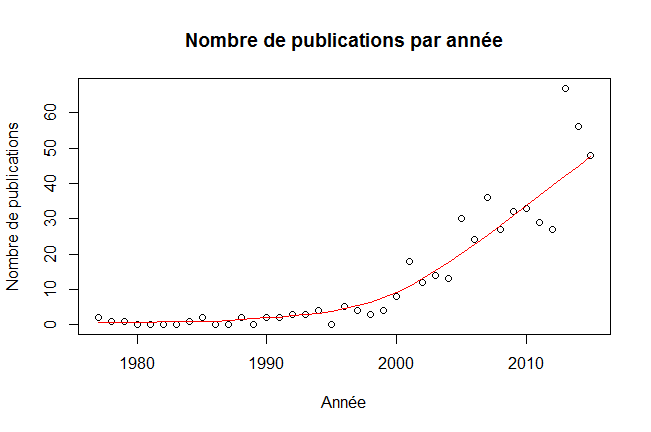
\includegraphics[scale=0.6]{Images/NbPerYear/NbPerYear}
\caption{Évolution du nombre d'articles publiés sur la modélisation du comportement des occupants}
\label{fig:NbPerYear}
\end{figure}

Le développement de modèles consiste à analyser les informations issues de la collecte et de formuler mathématiquement des lois qui en découlent. Pour rappel, un modèle permet de décrire un système en utilisant des concepts mathématiques. Il sert à prédire un état (\textit{output}) en fonction de variables explicatives (\textit{inputs}). La formulation d'un bon modèle répond à plusieurs principes: Elle est parcimonieuse, c'est à dire que les paramètres explicatifs sont statistiquement significatifs. Le modèle est basé sur des données de qualité (suffisantes, calibrées et complètes). Les outputs sont rigoureusement validés par validations croisées. Et enfin, le champ d'applicabilité est honnêtement déclaré.

Nous proposons dans cette section une revue succincte de trois formulations mathématiques fréquemment utilisées dans la modélisation du comportement des occupants, puis une présentation des méthodes d'évaluation de ces modèles.

\subsection{Formulations mathématiques}
\label{Formulations mathématiques}

Les trois formes majeures de modèles stochastiques pour représenter le comportement sont le processus de Bernoulli, les chaines de Markov et l'analyse de la survie. Le principe commun de ces formulations est de comparer une probabilité à un nombre aléatoire.

\subsubsection{Processus de Bernoulli}

Le processus de Bernoulli est un processus stochastique statique où la probabilité de l'état à prédire ne dépend pas de l'état précédent. Ce processus est une séquence de variables aléatoires indépendantes $\lbrace X_{t}:t=0,1,2,...n\rbrace$.  

$X_{t}$ est égal à 0 (l'évènement ne se produit pas) ou 1 (l'évènement se produit) pour toutes valeurs de $t$ dans le cas d'une prédiction binaire. Dans ce cas, une régression logistique binomiale est utilisée et la probabilité d'action est définit par:

\begin{equation}
P(x_{1}...x_{n}, t)=\frac{exp\left( \alpha + \sum\limits_{k=1}^n \beta_{k}x_{k}\right)}{1+exp\left( \alpha + \sum\limits_{k=1}^n \beta_{k}x_{k}\right)}
\end{equation}

avec $\alpha$ et $\beta_{k}$ l'intersection et la pente pour l'ensemble des n variables à expliquer.

Dans le cas où plus de deux résultats possibles sont à prédire, une régression logistique multinominale est utilisée, la probabilité d'action est alors définit par:

\begin{equation}
P_{j}(x, t)=\frac{exp (A_{j}(x))}{\sum\limits_{j=1}^n exp (A_{j}(x))}, j= 1, ..., N
\end{equation}
avec $A_{j}(x) = \alpha_{j} + \sum\limits_{j=1}^n \beta_{jk}x_{jk}$ et $N$ le nombre d'états.

\subsubsection{Chaine de Markov}
\label{Chaine de Markov}

Une chaîne de Markov $\lbrace X_{t}:t=0,1,2,...n\rbrace$ est un processus stochastique capable d'estimer l'état futur $X_{t+1}$ en fonction de l'état présent $X_{t}$ mais indépendamment des états passés $X_{0}, X_{1}, ..., X_{t-1}$. Elle ont l'avantage en comparaison avec le processus de Bernoulli de rendre la simulation plus fiable sur les transitions d'états. La probabilité de transition d'un état $i$ au pas de temps $t$ à un état $j$ au pas de temps $t+1$ $(T_{ij})$ peut être formulé comme:

\begin{equation}
T_{ij}(t)=P(X_{t+1}=j|X_{t}=i)
\end{equation}

On obtient alors la matrice de transition d'état $ T_{ij}(t)= \begin{bmatrix}
        T_{00}(t) & T_{01}(t) & \cdots & T_{0n}(t)\\
        T_{10}(t) & T_{11}(t) & \cdots & T_{1n}(t)\\
        \vdots & \vdots & \ddots & \vdots\\
        T_{n0}(t) & T_{n1}(t) & \cdots & T_{nn}(t)\\
     \end{bmatrix}$ pour $n+1$ états possibles.
     
Dans le cas d'un système binaire la matrice de transition $ T_{ij}(t)$ est réduite à 2 dimensions. La somme des probabilités d'une ligne étant égale à 1, il suffit de connaître deux probabilités de transition pour en déduire l'ensemble du système. La matrice réduite est donc $T_{ij}(t)= \begin{bmatrix}
        1-T_{01}(t) & T_{01}(t)\\
        1-T_{11}(t) & T_{11}(t)       
     \end{bmatrix}$

\subsubsection{Analyse de survie}

L'analyse de survie est un processus stochastique utilisé pour prédire la probabilité de durée d'un évènement. Plusieurs distributions paramétriques permettent de prédire ces durées de survie, dont la distribution de Weibull qui est la forme la plus générale. Sa densité de probabilité, ou taux de défaillance instantanée, est définit par la fonction: 
\begin{equation}
f(t) = \lambda p(\lambda t)^{p-1}e^{-(\lambda t)^{p}}
\end{equation}
avec le paramètre d'échelle $\lambda = 1/exp\left( \alpha + \sum\limits_{i=1}^k \beta_{i}x_{i} \right)$ et le paramètre de forme $log(1/p) $. Et sa fonction de survie par:
\begin{equation}
S(t) = P(T>t)=exp(-(\lambda t)^{p})
\end{equation}
A partir de la fonction de survie, lorsque l'état j commence, la durée correspondante peut être estimée en isolant $t$:
\begin{equation}
t_{j}=\frac{(-log(U))^{1/p}}{\lambda}
\end{equation}
avec $U$ un nombre aléatoire compris entre 0 et 1.

Nous pouvons noter que la distribution exponentielle peut aussi servir à l'analyse de la survie, et qu'elle est un cas particulier de la distribution de Weibull lorsque le paramètre de forme $p$ est égal à 1.

\subsection{Évaluation et validation}

Le développement de modèles résulte de campagne de mesures et d'analyses. Or, une étape fondamentale est parfois négligée, il s'agit de celle de validation des modèles. La majorité des processus de validations passés sont limités à la comparaison des sorties de la simulation aux données dans le même contexte que le modèle a été développé. Cela mène à une surestimation des performances du modèle. Cette section présente les approches de validation de modèles pour le comportement des occupants.

On recense deux types de validation; les procédures de validation internes et les procédures de validation externe. Steyerberg \cite{Steyerberg-03} définit les données externes comme des données venant de mesures différentes mais venant tout de même d'une population plausiblement liée.

Dans le contexte du comportement des occupants dans les bâtiments il y a au moins trois dimensions externes à considérer: le temps, l'environnement et les occupants. La question est alors de connaître quelles dimensions doivent varier pour obtenir des données externes. Si l'objectif du modèle est de modéliser un comportement dans un bâtiment particulier alors une variation dans le temps peut être suffisante pour l'obtention de données externes. Or si l'objectif du modèle est d'être généralisé à des occupants et à des bâtiments divers alors davantage de données issus d'autres occupants et d'autres bâtiments est nécessaire.
[Revisiting validation methods of OB models - Wolf - 2015]

\subsection{\textit{Fit-for-purpose} et facteurs contextuels}

Gaetani et al. \cite{Gaetani-16} proposent une méthodologie, appelée \textit{fit-for-purpose} permettant de sélectionner le modèle de comportement des occupants le plus approprié à l'objectif de l'utilisateur. Ce terme initialement proposé par Pitt and Myung \cite{Pitt-02} dans un contexte plus large d'analyse statistique met en garde sur la nécessité de développer des modèles qui sont ajustés aux objectifs de la modélisation. Un modèle sous-ajusté, et donc sous-paramétré, ne permet pas de reproduire le phénomène étudié, il sera alors trop rigide et ne permet pas de suivre les données. Alors qu'un modèle sur-ajusté, et donc sur-paramétré, prendra en compte des variations non-significatives et ne sera pas reproductible sur de nouvelles données. 

Yan et al. \cite{Yan-15} ont signalé dans leur article sur les futurs défis de la modélisation du comportement des occupants, que l'intégration des facteurs contextuels est un travail indispensable pour améliorer la reproductibilité des modèles. Dans la suite, nous proposons alors d'intégrer, lorsque le \textit{fit-for-purpose} n'est pas envisageable, un certain nombre de facteurs contextuels aux modèles les plus solides que nous avons préalablement identifiés.

Afin de mettre en évidence ces deux termes forts de cette thèse, la Figure de principe \ref{fig:Fit-to-purpose} met en avant la nécessité, d'une part de développer des modèles avec un niveau de complexité ni trop faible (a) ni trop élevé (c) pour obtenir des modèles parcimonieux mais néanmoins de proposer une mise en contexte des modèles afin qu'ils puissent être réutilisés pour un bâtiment autre que celui ayant servi à son développement. Ainsi, le modèle de principe utilisé dans le cadre (f) et issu du modèle (c), ne produit pas mieux les données que le modèle issu de (b) et réutilisé dans (e) malgré une qualité d'ajustement meilleure lors du développement du modèle.

\begin{figure}[H]
\centering
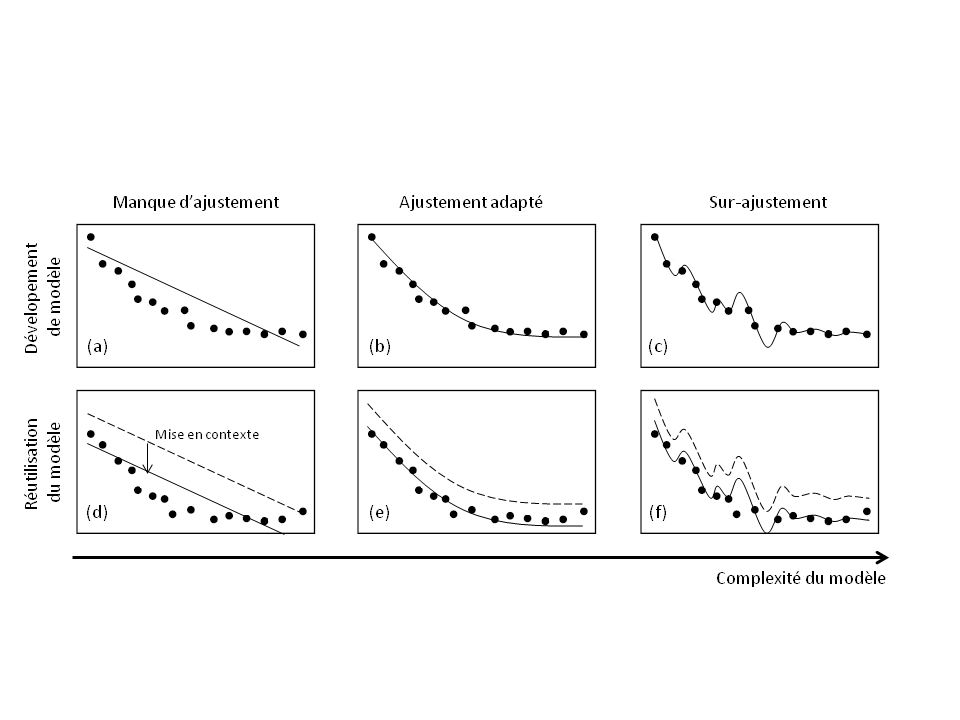
\includegraphics[scale=0.62]{Images/ComplexityAndContextualization}
\caption{Relation entre la qualité de l'ajustement (\textit{goodness of fit}), la complexité du modèle et la mise en contexte}
\label{fig:Fit-to-purpose}
\end{figure}

\section{Présentation des cas d'études}

Nous proposons dans cette section de présenter un bâtiment tertiaire virtuel et une maison individuelle conçue par l'Agence PY Architectes et notre bureau d'étude AI Environnement. Ces deux cas d'étude serviront à illustrer l'ensemble des modèles présentés plus loin dans ce chapitre. Le style architectural de ces cas d'étude est limité, en revanche les matériaux de construction sont très performants et la conception est proche d'une démarche passive.

Notre volonté initiale était de récupérer des données issues de projets réels suivi en phase d'exploitation afin de pouvoir comparer les résultats issus de nos simulations aux mesures in-situ et donc de travailler sur le \textit{performance gap}. Néanmoins, la confidentialité des documents espérés et les lenteurs administratives nous ont amené à revoir nos ambitions à la baisse. Ce changement de programme ne remet néanmoins pas en cause la co-simulation ou les modèles présentés ci-après.

\subsection{Bureau}

La Figure \ref{fig:CasEtudeBureau} représente le bâtiment de bureau, localisé en Gironde, utilisé lors des études portants sur le tertiaire. 

Par soucis de simplicité, nous avons opté pour des formes simples, nous n'avons pas intégré de masques proches ou lointains et nous avons orienté le bâtiment vers le sud. Le modèle comporte autant de zones que de pièces; 2 bureaux et un couloir. Le matériel de construction est synthétisé dans le Tableau \ref{tab:materialBureau}. Les ouvertures sont du triple vitrage argon 3/13/3/13/3 mm de coefficient de transmission thermique $U_{w}$ = 0.786 W/(m2.K). L'ensemble des ouvertures est équipé de système d'ombrage intérieur. Le renouvellement d'air est assuré par une ventilation mécanique double flux de rendement 70 \% et l'étanchéité à l'air est fixée à taux constant (pas de prise en compte météorologique) à $n_{50}$ = 0.150 Vol/h. Le bâtiment est chauffé électriquement et n'a pas de système de refroidissement actif.

\begin{figure}[H]
\centering
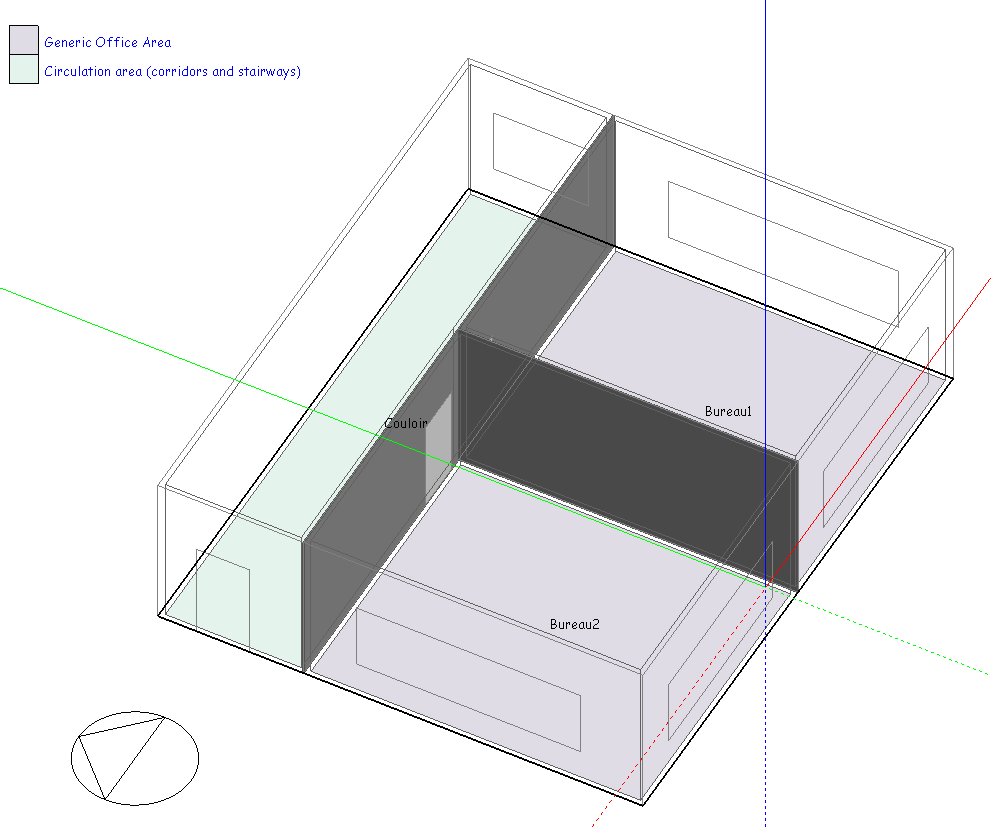
\includegraphics[scale=0.55]{Images/CasEtudeBureau}
\caption{Modèle 3D des 2 bureaux virtuels, vue du sud/ouest sous DesignBuilder}
\label{fig:CasEtudeBureau}
\end{figure}

\begin{center}
\begin{table}
\begin{tabular}{|c|c|c|c|c|}
\hline 
Construction & Couches & Épaisseur (cm) & Matériaux & U [W/(m2.K)] \\ 
\hline
\hline \multirow{3}*{Murs extérieurs} & Externe & 0.6 & Bardage métallique & \multirow{3}*{0.132} \\ 
\cline{2-4}  & 2 & 25 & Polystyrène XPS extrudé &  \\ 
\cline{2-4}  & Interne & 1.3 & Plâtre &  \\ 
\hline \multirow{4}*{Toiture} & Externe & 1 & Asphalte & \multirow{4}*{0.151} \\ 
\cline{2-4}  & 2 & 25 & Laine de verre &  \\ 
\cline{2-4} & 3 & 20 & Lame d'air &  \\ 
\cline{2-4} & Interne & 1.3 & Placoplâtre &  \\ 
\hline \multirow{2}*{Plancher} & Externe & 15 & Polystyrène XPS extrudé & \multirow{2}*{0.208} \\ 
\cline{2-4}  & Interne & 15 & Béton coulé &  \\ 
\hline \multirow{3}*{Cloisons intérieures} & Externe & 2.5 & Plaque de plâtre & \multirow{3}*{1.923} \\ 
\cline{2-4} & 2 & 10 & Lame d'air &  \\ 
\cline{2-4} & Interne & 2.5 & Plaque de plâtre &  \\ 
\hline 
\end{tabular} 
\caption{Composition et caractéristiques des matériaux de construction du bâtiment de bureau}
\label{tab:materialBureau}
\end{table}
\end{center}

\subsection{Résidentiel}

La Figure \ref{fig:CasEtudeBureau} représente la modélisation d'une maison individuelle suivant une démarche passive dans le bassin d'Arcachon à Andernos-les-Bains. Cette maison compacte est choisie comme cas d'étude pour cette thèse, car elle offre une architecture simple et performante, répondant à nos besoins de recherche. Cette compacité ne remet pas en cause les possibilités de l'outil à modéliser des cas plus complexes, mais elle a l'avantage de réduire les temps de développement et de calcul. Le découpage en zones thermiques mène à 6 zones distinctes, la buanderie ayant été intégrée au séjour et le point d'eau de la chambre ayant été transféré à la salle de bain principale (Figure \ref{fig:PlanMaison}).

Le fichier météo, issu de la base de données EnergyPlus, ayant servi à la simulation est le fichier FRA\_Bordeaux.075100\_IWEC.epw obtenu sur des mesures, sur le site de Bordeaux-Mérignac, comprises entre 1983 et 1999, suivant la procédure de création de fichiers détaillée à la section \ref{Météo}. Les caractéristiques de l'enveloppe sont présentées dans le Tableau \ref{tab:materialMaison}. Comme pour le cas de bureaux, les ouvertures sont du triple vitrage argon 3/13/3/13/3 mm de coefficient de transmission thermique $U_{w}$ = 0.786 W/(m2.K). L'ensemble des ouvertures est équipé de système d'ombrage intérieur. Le renouvellement d'air est assuré par une ventilation mécanique double flux de rendement 70 \% et l'étanchéité à l'air est fixé à taux constant (pas de prise en compte météorologique) à $n_{50}$ = 0.200 Vol/h. Le bâtiment est chauffé au gaz naturel et n'a pas de système de refroidissement actif.

\begin{figure}[H]
\centering
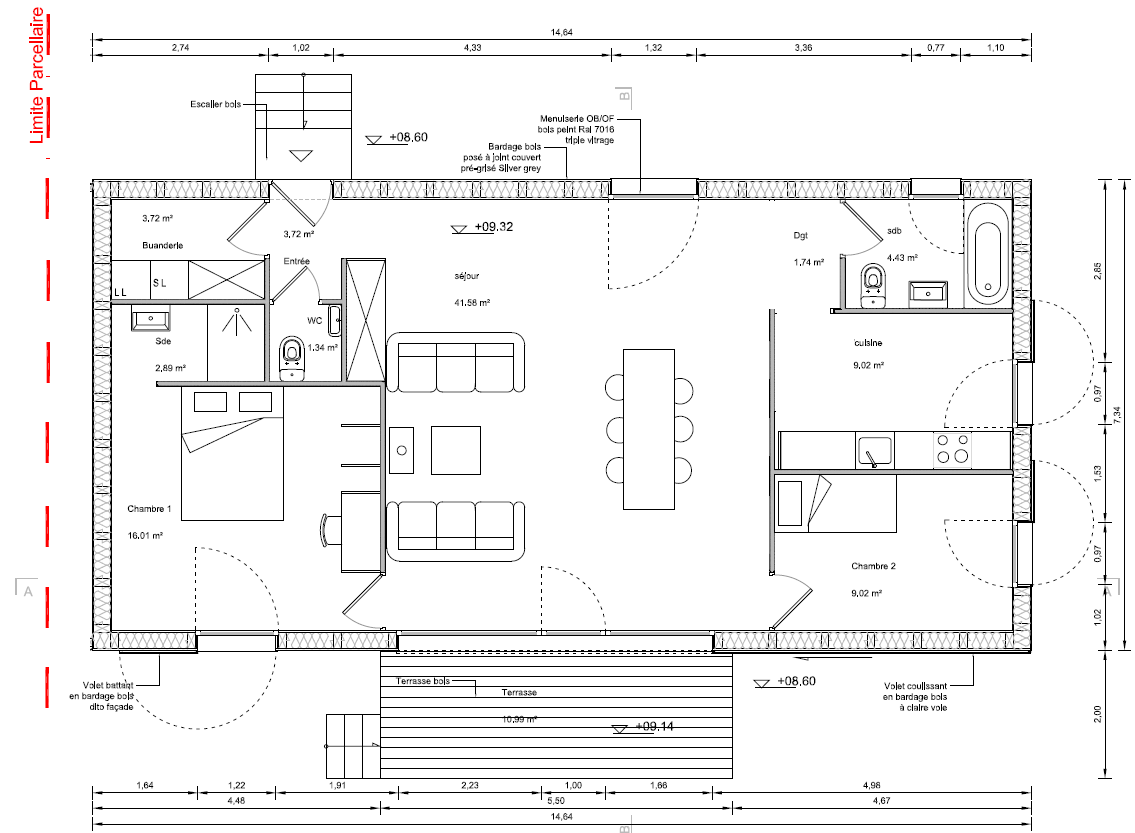
\includegraphics[scale=0.55]{Images/PlanMaison}
\caption{Plans architecte de la maison à Andernos-les-bains}
\label{fig:PlanMaison}
\end{figure}

\begin{figure}[H]
\centering
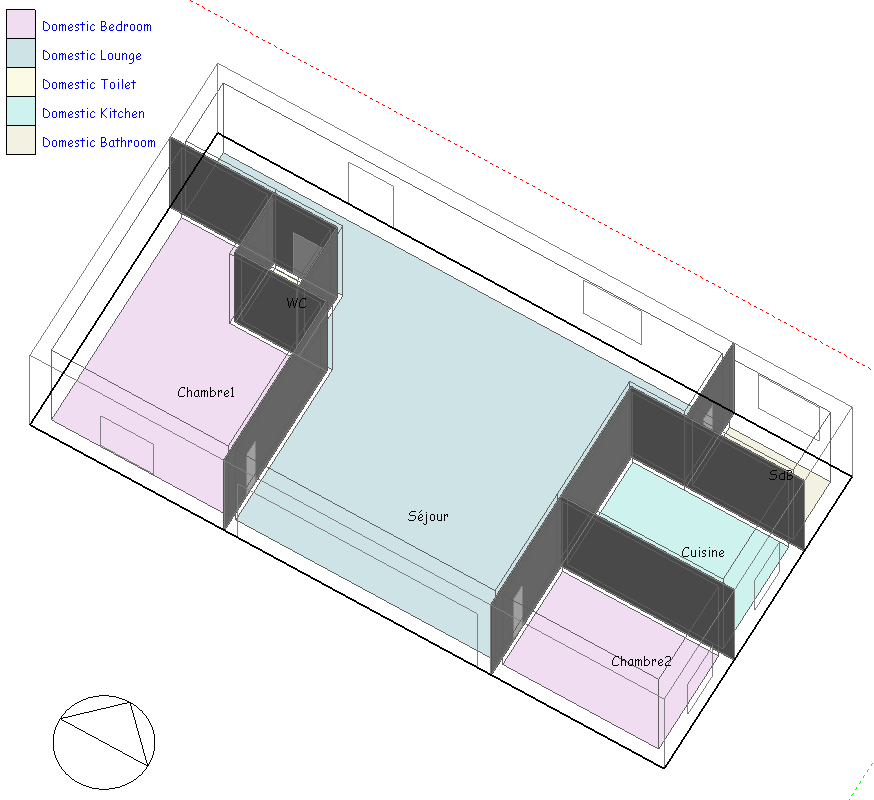
\includegraphics[scale=0.55]{Images/CasEtudeMaison}
\caption{Modèle 3D de la maison construite à Andernos, vue du sud/est sous DesignBuilder}
\label{fig:CasEtudeMaison}
\end{figure}

\begin{center}
\begin{table}
\begin{tabular}{|c|c|c|c|c|}
\hline 
Construction & Couches & Épaisseur (cm) & Matériaux & U [W/(m2.K)] \\ 
\hline
\hline \multirow{3}*{Murs extérieurs} & Externe & 1 & Enduit extérieur & \multirow{3}*{0.121} \\ 
\cline{2-4}  & 2 & 27.9 & Fibres végétales / Ossature bois &  \\ 
\cline{2-4}  & Interne & 1 & Plâtre &  \\ 
\hline \multirow{2}*{Toiture} & Externe & 35 & Panneaux de laine de verre & \multirow{2}*{0.102} \\ 
\cline{2-4} & Interne & 1 & Support métallique &  \\ 
\hline \multirow{3}*{Plancher} & Externe & 30.4 & Sol terreux & \multirow{3}*{0.376} \\ 
\cline{2-4} & 2 & 30.9 & Panneaux de laine de verre &  \\ 
\cline{2-4}  & Interne & 15 & Béton coulé &  \\ 
\hline \multirow{3}*{Cloisons intérieures} & Externe & 1.3 & Plaque de plâtre & \multirow{3}*{2.358} \\ 
\cline{2-4} & 2 & 10 & Lame d'air &  \\ 
\cline{2-4} & Interne & 1.3 & Plaque de plâtre &  \\ 
\hline 
\end{tabular} 
\caption{Composition et caractéristiques des matériaux de construction de la maison}
\label{tab:materialMaison}
\end{table}
\end{center}

\section{Présence dans les bâtiments de bureaux}

A RÉDIGER------------->: Les bâtiments accueillant des activités autres que de bureau et résidentiel, tels que les centres commerciaux, les établissement scolaires ou les musées ne sont pas modélisé car suivant des horaires de travail réguliers et spécifiques

\label{PresenceBureau}

Les scénarios de présence dans les bureaux et d'activités dans les logements constituent une entrée indispensable pour les modèles adaptatifs (gestion de température de consigne, fenêtres, stores et volets, éclairage) et non adaptatifs (utilisation d'appareils électriques, consommation d'eau chaude). Nous proposons donc dans ce chapitre et le suivant de considérer deux familles de modèles de prédiction des activités, d'une part les présences et absences dans les bâtiments de bureaux et d'autre part les activités dans les logements. Cette distinction fondamentale également partagée par plusieurs chercheurs \cite{Vorger-14}, \cite{Page-08}, \cite{Chapman-14} peut être vue comme un \textit{fit-for-purpose} dans le sens ou les modèles sont radicalement différents et n'ont pas de racines communes.

Bien que les horaires de travail et les horaires d'occupation des logements soient très corrélés pour l'ensemble de la population, les deux modèles présentés dans ce chapitre et dans le chapitre \ref{ActivitésLogements} sont totalement indépendant. Nous justifions ce choix par une modélisation dans cette thèse à l'échelle du bâtiment. Une modélisation plus large à l'échelle du quartier ou de la ville impliquerait alors une approche ou les activités professionnelles et privées seraient dépendantes.

L'objectif de ce chapitre est de proposer un modèle qui reproduit plus fidèlement la présence de travailleurs de bureaux que les scénarios conventionnels couramment utilisés. Le modèle proposé dans ce chapitre est définit en pré-processus de la simulation, c'est à dire qu'il est connu pour l'ensemble de la simulation avant que celle-ci n'ai débutée. Ce choix se justifie par la non-nécessité, à priori, de connaître les variables environnementales pour définir les horaires de travail. La première partie de cette section présente un état de l'art des modèles stochastiques de présence dans les bureaux et plus particulièrement le modèle de Page et al. \cite{Page-08} qui est utilisé comme base dans la suite. La seconde partie présente comment ce modèle développé sur des bureaux universitaires de chercheurs peut être également appliqué sur des bureaux privés. Enfin, une présentation des résultats de ce modèle et de ces sous-modèles est proposée.

\subsection{État de l'art}

Afin d'établir des modèles stochastiques réalistes de présence dans les bureaux pour associer une présence à des apports métaboliques et à des actions possibles plusieurs travaux ont été réalisés. Le Tableau \ref{tab:PresencePresentation} et \ref{tab:PresenceOffice} présentent respectivement le contexte du développement des modèles et leurs variables d'entrée et de sortie. Nous présentons avant cela les modèles les plus pertinents. 

En 1995, Newsham et al. \cite{Newsham-95} ont proposé un premier modèle probabiliste de présence simple afin de créer des scénarios d'occupation dans le cadre du travail de modélisation de la gestion de l'éclairage artificielle, lightswich. En 2003, Yamagushi et al. \cite{Yamaguchi-03} ont également développé un modèle de présence simple grave à des chaines de Markov, servant d'entrée à la prédiction de la demande d'énergie à l'échelle d'un quartier. Ces deux modèles étant très simplifiés ils ne seront pas présentés plus en détails dans les tableaux suivant.

Wang et al. \cite{Wang-05} ont examiné les propriétés statistiques d'occupation dans des bureaux individuellement occupés. Ils ont réalisé l'hypothèse que les durées des périodes de présences et d'absences intermédiaires sont distribuées exponentiellement et que le coefficient de la distribution peut être traité comme une constante sur la journée. Aussi, ils proposent de générer les premières arrivées, les premiers départs et les pauses déjeuners en assumant que ces périodes suivent une loi normale. Bien qu'élégant, ce modèle ne permet de reproduire la complexité de de présence réelle et sur-estiment la présence, tout comme les scénarios conventionnels.

Page et al. \cite{Page-08} proposent un modèle basé sur des chaines de Markov à deux états à partir d'une campagne de mesure longue sur 5 bureaux universitaire à Lausanne. Ce modèle est capable de reproduire les caractéristiques d'occupations, comme les arrivées, les départs, les absences intermédiaires et les absences longues, mais il n'est pas capable de simuler les mouvements entre les zones. Néanmoins, ce modèle est très probablement celui qui a été le plus repris dans des travaux postérieurs, notamment par Liao et al. \cite{Liao-11}, Vorger \cite{Vorger-14} et Feng et al. \cite{Feng-15}, avec de bonnes capacités de prédiction.

Erickson et al. \cite{Erickson-09} ont utilisé les données collectées d'occupation de bureaux pour développer un modèle basé sur des lois Gaussienne multidimensionnelles aux périodes de transitions. Ce modèle a par la suite été intégré dans un modèle à base d'agents dans le but de prédire la mobilité sur plusieurs zones des agents. Cependant, les résultats montrent une faible reproduction des mesures, de l'ordre de 20 \%.

Tabak et de Vries \cite{Tabak-10} ont généré des profils d'occupation basés sur l'enchainement chronologique des activités des occupants. Cette approche détaillée reproduit bien la complexité du comportement des occupants mais nécessite un gros travail de questionnaires et de mesures. Cette méthode indirecte est plus complexe à intégrer dans un outil de simulation que les autres approches mentionnées précédemment.

Davis et Nutter \cite{Davis-10} ont instrumenté 6 type de bâtiments universitaire aux activités différentes afin de proposer des profils de présence hebdomadaire selon ces familles d'activités. Les résultats synthétisent les probabilités de présence par type de bâtiment et il a été conclu que les jours de la semaines sont parfois significativement différents.

Liao et al. \cite{Liao-11} proposent un modèle permettant de suivre la location des occupants dans l'espace et dans le temps. Ce modèle puissant permet une bonne prédiction de l'occupation dans le cas de faible nombre de zone mais une prédiction approximative dans le cas de multi-zones. Les auteurs indiquent que la configuration du modèle est très chronophage et difficilement extensible.

Wang et al. \cite{Wang-11} utilisent une modélisation de la présence dans les bâtiments de bureaux basée sur les chaines de Markov à niveaux multiples. Le nombre de niveaux correspond au nombre de zones où l'agent est susceptible de se trouver. Ces travaux sont bien documentés mais relèvent plus d'une méthodologie qu'une proposition de modèle calibré, car les résultats ne sont pas issus de campagne de mesures ou d'enquêtes.

Duarte et al. \cite{Duarte-13} ont collecté réalisé une campagne longitudinale pour montrer les variations des facteurs d'occupation dans des bâtiments de bureaux selon l'heure de la journée, le jour de la semaine et le mois de l'année. Les comparaisons ont montré une variabilité élevée entre ces paramètres et un écart de la moyenne de 46 \% inférieur au standard américain ASHRAE 90.1. Ce travail met également en avant la variabilité des profils de présence en fonction des vacances et du type d'espace, notamment entre les bureaux privés et les bureaux partagés.

Chang et Hong \cite{Chang-14} ont analysé 200 bureaux cubiques de 3 étages aux activités différentes d'un bâtiment commercial. Un modèle mathématique est proposé afin de décrire le nombre et la durée des périodes d'absences. Une première fonction de densité cumulée (\textit{CDF}) définit le nombre d'absence, une seconde fonction de densité cumulée définit la durée et une distribution de probabilité (\textit{PDF}) définit le début d'une période d'absence. Les auteurs ont identifié des profils d'occupation groupés en 5 catégories prouvant la variabilité de présence.

Feng et al. \cite{Feng-15} ont développé un modèle d'occupation inspiré du modèle de Wang et al. \cite{Wang-11} qu'ils ont couplé à un logiciel de simulation thermique. Ce modèle est une chaine de Markov à 12 niveaux correspondant aux 12 zones du cas d'étude. Quelques hypothèses sont présentées dans l'article concernant les activités des différents membres du bâtiment. Il est ainsi avancé que les managers sont moins présent dans les bureaux que les chercheurs pour assister à des conférences ou participer à des réunions, cela menant à une présence dans leurs propres bureaux moins importante.

Mahdavi et Tahmasebi \cite{Mahdavi-15} ont testé 3 modèles d'occupation sur des données issues de mesures sur une Université de Vienne. Les deux premiers modèles d'occupation sont stochastiques, il s'agit du modèle proposé par Reinhart \cite{Reinhart-01} (non-détaillé ici) et celui de Page et al. \cite{Page-08}. Le troisième modèle est un modèle non-probabiliste d'apprentissage qui génère des profils d'occupation binaire journalière basés sur les données de présence passées. Une fois la phase d'apprentissage suffisamment robuste, la phase d'évaluation montre que le modèle non-stochastique prédit mieux la présence que les modèles stochastiques.

\begin{landscape}
\begin{table} [H]
\begin{tabular}{|p{2.5cm}|p{2cm}|p{2cm}|p{2cm}|p{2cm}|p{2cm}|p{4cm}|p{4cm}|}
\hline 
Auteurs & Location & Bâtiment & Durée campagne & Intervalle de mesure & Modèle & Points forts & Points faibles \\ 
\hline 
\hline
Wang et al. \cite{Wang-05}, 2005 & USA & 35 bureaux & 1 année & 15 minutes & Processus de Poisson & Présence intermédiaire modélisé; Simplicité du modèle & Bureau unique \\ 
\hline 
Page et al. \cite{Page-08}, 2008 & Suisse & 20 zones universitaires (10 bureaux) & 2 années & 15 minutes & Chaine de Markov & Détaillé pour implémentation; comparé postérieurement & Données d'entrée complexes; Sous-estimation du nombre de jour d'absence total \\ 
\hline 
Ericksen et al. \cite{Erickson-09}, 2009 & USA & 4 zones universitaires & 2 fois 1 jour & Vidéo & Multivarié Gaussien & Comparaison de modèles sur différentes zones & Durée de la campagne; Erreur des modèles importante  \\ 
\hline 
Tabak et de Vries \cite{Tabak-10}, 2010 & Pays-bas & 1 bureau (8 occupants enquêtés) & - & - & S-curve; Méthode probabiliste & Prédiction d'activités intermédiaires  & Modèle basé sur des questionnaires uniquement \\ 
\hline 
Davis et Nutter \cite{Davis-10}, 2010 & USA & 11 bâtiments universitaires & 5 mois & Vidéo & - & Identification de facteurs par type de bâtiment & Pas de modèle proposé \\ 
\hline 
Liao et al. \cite{Liao-11}, 2011 & USA & Bâtiment commercial & - & 15 minutes & Chaine de Markov & Comparaison de modèle & Campagne de mesure très peu présenté \\ 
\hline 
Wang et al. \cite{Wang-11}, 2011 & - & 5 bureaux & - & 5 minutes & Chaine de Markov à 7 niveaux & Suivi zone par zone des occupants & Modèle non-basé sur des mesures \\ 
\hline 
Duarte et al. \cite{Duarte-13}, 2013 & USA & Bâtiment commercial & 2 années & 1 minute & Modèle déterministe & Large campagne de mesures reflétant l'influence de facteurs contextuels & Pas de modèle clairement proposé \\ 
\hline 
Chang et Hong \cite{Chang-14}, 2014 & Taiwan (?) & 200 bureaux & 6 mois & 5 minutes & Fonction de distribution cumulative et de probabilité & Groupement suivant 5 familles de profils & Modèle applicable à des bureaux non-partagés \\ 
\hline 
Feng et al. \cite{Feng-15}, 2015 & - & 12 zones universitaires & - & - & Chaine de Markov à 12 niveaux  & Suivi zone par zone des occupants & Modèle non-basé sur des mesures \\ 
\hline 
Mahdavi et Tahmasebi \cite{Mahdavi-15}, 2015 & Autriche & 8 zones universitaires & 9 mois & 15 minutes & Modèle d'apprentissage & Comparaison de modèles & Profil d'occupation unique \\ 
\hline 
\end{tabular}
\caption{Synthèse des modèles les plus pertinents de présence et d'activités dans les bureaux}
\label{tab:PresencePresentation}
\end{table}
\end{landscape}

\begin{table} [H]
\centering
\begin{tabular}{|l||c|c|c|c|c|c|c|c|c|c|c|}
\hline
\textbf{Variables\textbackslash Auteurs} & \cite{Wang-05} & \cite{Page-08} & \cite{Erickson-09} & \cite{Tabak-10} & \cite{Davis-10} & \cite{Liao-11} & \cite{Wang-11} & \cite{Duarte-13} & \cite{Chang-14} & \cite{Feng-15} & \cite{Mahdavi-15} \\
\hline
\hline \rowcolor{gray}\textbf{Environnementales} & \multicolumn{11}{c}{} \\
\hline Mois/Saison &  &  &  &  &  &  &  & X &  &  &   \\
\hline Météo & / &  &  &  &  &  &  & / & / &  &   \\
\hline \rowcolor{gray}\textbf{Contextuelles} & \multicolumn{11}{c}{} \\
\hline Heure de la journée & X & X & X & X & X & X & X & X & X & X & X \\
\hline Type d'activité &  &  &  & X & X & X & X &  & X & X &  \\
\hline Jour de la semaine &  & X &  & X & X & X &  & X &  &  &   \\
\hline Activités intermédiaires &  &  &  & X &  & / & X &  &  &  &   \\
\hline \rowcolor{gray}\textbf{Bâtiment} & \multicolumn{11}{c}{} \\
\hline Type de zones &  &  & X &  & X &  & X & X &  & X &   \\
\hline \rowcolor{gray}\textbf{A expliquer} & \multicolumn{11}{c}{} \\
\hline Statut d'occupation & X &  &  &  &  &  &  &  & X &  &   \\
\hline Nombre d'occupant par zone &  & X &  &  & X &  &  & X &  &  & X  \\
\hline Location des occupants &  &  & X & X &  & X & X &  &  & X &   \\
\hline
\end{tabular}
\caption{Synthèse des données d'entrée et de sortie des modèles de présence et activités dans les bureaux}
\label{tab:PresenceOffice} 
\end{table}

Conclusions/Discussion/Choix du modèle:
\begin{itemize}
\item
\item Certains modèles permettent de prendre en compte les déplacements entre plusieurs zones du bâtiment. Toujours constitués de chaines de Markov le modèle gagne en réalisme mais s'en trouve alourdi. De plus, il est alors nécessaire de donner en entrée du modèle la probabilité de présence de chaque occupant, dans chaque zone et à chaque pas de temps
\end{itemize}

\subsection{Modèle de Page}

----
Le modèle initial ayant été développé dans un contexte universitaire, il n'est à priori pas nécessairement valide pour des bâtiment de bureaux abritant d'autres activités, les horaires de travail dépendant des catégorie socio-professionnelles. Une solution consiste à répliquer le travail de Page et al. \cite{Page-08} pour plusieurs typologies de bâtiments afin de calibrer le modèle de base. Un ajustement contextuel plus fin serait ensuite possible afin de considérer davantage de facteurs influents. Dans la suite, nous utiliserons uniquement le modèle de Page comme base ajustable, car ce modèle est le plus robuste de notre base bibliographique et en développer davantage reste un travail coûteux et chronophage. Néanmoins, afin de rendre ce modèle applicable à une gamme de bâtiments et un type d'occupants plus large, nous proposons d'y ajouter des facteurs contextuels rendant l'ensemble plus flexible et plus approprié.
----


Comme nous venons de le voir, les chaînes de Markov permettent de reproduire des transitions d'états et donc de rendre la dynamique de simulation plus cohérente avec les présences et absences des occupants. La section \ref{Chaine de Markov} a présenté le fonctionnement de base des chaînes de Markov. Page et al. \cite{Page-08} ont proposé un modèle de transition d'état pour les bâtiments de type bureau utilisant des chaînes de Markov. Sur la base de mesures de présence dans 5 bureaux de l'Ecole Polytechnique Fédérale de Lausanne pendant 4 ans, Page et al. ont proposé des probabilités de présence heure par heure pour une semaine type, soit 168 (24*7) probabilités. 

Les probabilités de transitions $T_{ij}(t)$ sont calculés à partir des probabilités de présence et l'équation suivante en est déduite:

\begin{equation}
T_{11}(t)=\dfrac{P(t)-1}{P(t)}T_{01}(t)+\dfrac{P(t+1)}{P(t)}
\label{T110}
\end{equation}

Néanmoins, une information est manquante pour déterminer les valeurs $T_{01}$ et $T_{11}$ à chaque pas de temps. Les auteurs ont alors défini un paramètre de mobilité:

\begin{equation}
\mu(t)=\dfrac{T_{01}(t)+T_{10}(t)}{T_{00}(t)+T_{11}(t)}
\label{mu}
\end{equation}

Pour simplifier les entrées du modèle et le calibrer, les auteurs ont fixé ce paramètre de mobilité ($\mu$) à 0.11. Cette valeur correspond à la valeur moyenne observée du paramètre de mobilité. Nous pouvons noter que plus $\mu$ est grand plus la transition d'état est fréquente.
A partir des équations \eqref{T110} et \eqref{mu} on peut alors déterminer les quatre probabilités de transition pour chaque pas de temps:

\begin{itemize}
\item $T_{01}(t)=\dfrac{\mu-1}{\mu+1}P(t)+P(t+1)$
\item $T_{00}(t)=1-T_{01}(t)$
\item $T_{11}(t)=\dfrac{P(t)-1}{P(t)}\left[\dfrac{\mu-1}{\mu+1}P(t)+P(t+1)\right]+\dfrac{P(t+1)}{P(t)}$
\item $T_{10}(t)=1-T_{11}(t)$
\end{itemize}

Il est à noter que pour certaines conditions, lorsque les probabilités de présence entre deux pas de temps $P(t)$ et $P(t+1)$ sont très différentes, la probabilité de transition $T_{ij}$ puisse ne pas être comprise entre 0 et 1. Dans ce cas, le paramètre de mobilité est modifié de tel façon à ce qu'il permettent à la probabilité de transition de prendre une valeur cohérente.

Lors du pré-processus de la simulation, la présence est calculés à partir des équations ci-dessus, afin d'être utilisée lors de la simulation. Pour ce faire, à chaque pas de temps un nombre aléatoire $rand$ compris entre 0 et 1 est généré par une loi uniforme, puis comparé à la probabilité de transition $T_{01}(t)$ si l'occupant est absent et à $T_{11}(t)$ si l'occupant est présent. Si $rand < T_{01}(t)$ alors l'occupant rentre dans la pièce, sinon non, et si $rand < 1-T_{11}(t)$ alors l'occupant sort dans la pièce, sinon il y reste.

Le Tableau \ref{tab:PPage} présente les probabilités de présence $P$, pour les lundis et pour les samedis, issues des mesures sur les 5 bureaux du modèle de Page et al. \cite{Page-08}. Les probabilités de présence du lundi sont représentatives de celles des jours de travail (lundi à vendredi), alors que les probabilités du samedi sont semblables à celles du dimanche. Les sorties du modèle de base sont présentés dans la section \ref{Facteurs contextuels} avec les variantes.

\begin{table}[H]
\centering
\begin{tabular}{|c|c|c|c|c|c|c|c|c|c|c|c|}
\hline 
Heure & 1 & 2 & 3 & 4 & 5 & 6 & 7 & 8 & 9 & 10  \\ 
\hline 
$P_{Lundi}$ & 0.021 & 0.021 & 0.021 & 0.021 & 0.021 & 0.021 & 0.021 & 0.025 & 0.250 & 0.422  \\ 
\hline 
$P_{Samedi}$ & 0.028 & 0.030 & 0.029 & 0.029 & 0.030 & 0.029 & 0.029 & 0.030 & 0.030 & 0.030  \\ 
\hline
\hline
Heure & 11 & 12 & 13 & 14 & 15 & 16 & 17 & 18 & 19 & 20 \\ 
\hline 
$P_{Lundi}$ & 0.309 & 0.377 & 0.187 & 0.375 & 0.426 & 0.396 & 0.375 & 0.432 & 0.084 & 0.070 \\ 
\hline 
$P_{Samedi}$ & 0.035 & 0.037 & 0.030 & 0.032 & 0.041 & 0.045 & 0.042 & 0.034 & 0.035 & 0.032 \\ 
\hline 
\hline
Heure & 21 & 22 & 23 & 24 & \cellcolor{lightgray}& \cellcolor{lightgray}& \cellcolor{lightgray}& \cellcolor{lightgray}& \cellcolor{lightgray}& \cellcolor{lightgray}\\ 
\hline 
$P_{Lundi}$ & 0.047 & 0.039 & 0.038 & 0.038 & \cellcolor{lightgray} &\cellcolor{lightgray} &\cellcolor{lightgray} &\cellcolor{lightgray} &\cellcolor{lightgray} & \cellcolor{lightgray}\\ 
\hline 
$P_{Samedi}$ & 0.027 & 0.024 & 0.021 & 0.021 &\cellcolor{lightgray} &\cellcolor{lightgray} &\cellcolor{lightgray} & \cellcolor{lightgray}&\cellcolor{lightgray} &\cellcolor{lightgray} \\
\hline 
\end{tabular}
\caption{Probabilités de présence dans les bureaux pour les lundis et les samedis}
\label{tab:PPage}
\end{table}

\subsection{Ajustement du modèle de Page et al.}
\label{AjustementPage}

Une fois le modèle brut de Page et al. \cite{Page-08} reprit dans la plateforme MASS, nous comparons nos résultats issus d'une simulation d'un an, d'un occupant et au pas de temps de 5 minutes avec ceux des auteurs pour vérifier la bonne programmation. Plusieurs observations nous amènent à proposer un ajustement du modèle de base. Celles-ci sont de deux types, d'une part les observations communes entre les codes, mais en contradiction avec nos connaissances socioprofessionnelles. Et d'autre part, des différences suffisamment significatives, entre la base et le modèle codé dans MASS, pour être rapportées ici.

La comparaison des profils de probabilités de présence est un premier bon indicateur de la qualité du modèle, la Figure \ref{fig:ProfilPresence} permet de constater une bonne reproduction globale, mais une présence semble t-il légèrement plus élevée les nuits dans notre cas. La Figure \ref{fig:ChronogrammeBase} est un chronogramme sur une année de simulation, les zones noires représentent les périodes travaillées et les zones grises les absences. Nous identifions clairement les matins et les après-midis comme périodes principalement travaillées, mais nous pouvons surtout noter des présences régulières courtes les nuits et confirmer notre impression issue du profil de présence.

\begin{figure}[H]
\centering
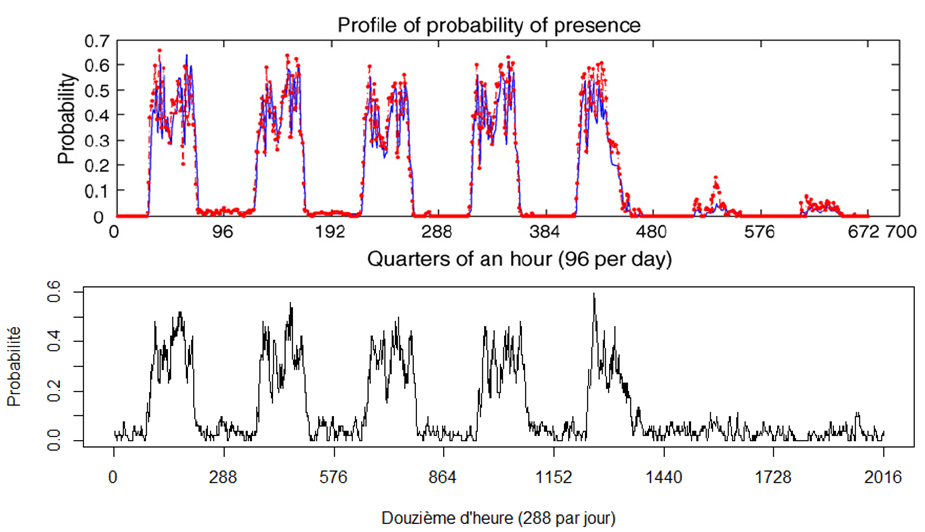
\includegraphics[scale=0.6]{Images/PageActivities/ProfilPresence}
\caption{Profils de présence mesuré (bleu) et simulé (rouge) issus de l'article de Page et al \cite{Page-08} (en haut) et généré dans la plateforme MASS (en bas)}
\label{fig:ProfilPresence}
\end{figure}

\begin{figure}[H]
\centering
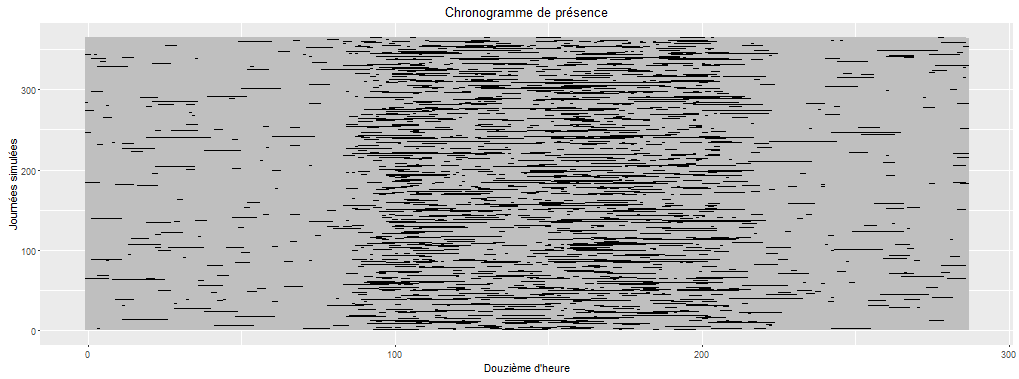
\includegraphics[scale=0.46]{Images/PageActivities/ChronogrammeBase}
\caption{Chronogramme de présence d'un agent sur un an selon le modèle initial de Page et al \cite{Page-08}}
\label{fig:ChronogrammeBase}
\end{figure}

Le second indicateur exploitable est la durée de présence dans les locaux. Dans l'article de Page et al. \cite{Page-08} une incohérence semble apparaitre. En effet, la durée de présence hebdomadaire moyenne est donnée à 24 heures soit 4h48 par jour, alors que la durée de présence quotidienne est quant à elle aux alentours de 9h par jour si l'on se fie aux graphiques. Sur une base de 5 jours de travail nous aboutissons dons à un décalage d'un facteur proche de 2. De notre côté, notre simulation nous amène à une durée moyenne de 3h49 et un écart-type de 1h24 sur les 5 jours travaillés, soit 1h de moins que la durée hebdomadaire du modèle de base.

Trois indicateurs complémentaires sont utilisés pour évaluer le modèle: l'heure de première arrivée, l'heure de dernier départ et le nombre de transitions d'états. Sur la base d'une simulation d'une année la moyenne d'heure de première arrivée est à 6h51, la médiane à 7h25 et l'écart type de 4h16, contre une médiane à 7h30 dans \cite{Page-08}. Ces résultats se justifient par la haute fréquence de présence de nuit déjà discuté en début de paragraphe. La moyenne d'heure de dernier départ est quant à elle à 17h58, la médiane à 17h50 et l'écart type de 3h56, contre une moyenne de 17h30 dans \cite{Page-08}. Le nombre moyen de transitions quotidien par jour à priori travaillé est de 12.60 et en semaine, week-end compris de 9.97, contre 8 dans \cite{Page-08}.

L'étude du modèle de base nous amène à deux remarques. D'une part le modèle produit une présence dans les bureaux trop importante les nuits et d'autre part la présence moyenne est sous-estimée par le modèle. Pour palier à ces remarques nous proposons de borner arbitrairement le modèle entre 5h et 21h, car nous estimons une présence à l'extérieure de ces bornes comme irréaliste pour un travail de bureau. De plus, afin de se caler sur les durées moyennes de travail hebdomadaire recensés par les organisations nationales de l'OECD\footnote{L'Organisation de Coopération et de Développement Économique est une organisation internationales d'études économiques - Site internet \url{http://www.oecd.org/fr/}} \cite{OECD-14} et de la DARES\footnote{La Direction de l'Animation de la Recherche, des Etudes et des Statistiques} \cite{Pak-13} qui sont données respectivement à 36h17 (2014) et 36h36 (2013), nous ajoutons un coefficient aux probabilités de présence $P(t)$. La durée moyenne de travail hebdomadaire issue de notre simulation étant de 20h31 nous pourrions proposer un coefficient de $(36h26/20h31=36.43/20.52=)1.78 $. Or, les durées issues du modèle correspondent à une présence effective dans les bureaux, contrairement aux durées tirées des études statistiques  qui sont des durées travaillées au bureau, mais également en déplacement, en réunion ou en télétravail, nous utiliserons dans la suite un ajustement des coefficients de présence abaissé à $1.7$ du lundi au vendredi de 5h à 21h. Les résultats du modèle ajusté sont présentés dans la section \ref{Facteurs contextuels} avec les modèles contextualisés.

\subsection{Facteurs contextuels}
\label{Facteurs contextuels}

Le modèle de Page et al.\cite{Page-08} est calibré sur des mesures de présence de bureaux individuels universitaires en Suisse. Il n'est alors pas nécessairement approprié pour reproduire la présence dans des bureaux de types différents dans des pays de cultures différentes. La solution la plus fiable, mais aussi la plus délicate à mettre en œuvre pour des raisons de moyen consiste à répliquer le travail réalisé par Page et al.\cite{Page-08} dans de nouveaux bâtiments de bureaux accueillant des travailleurs aux activités diverses. Ainsi, en fonction du bâtiment tertiaire à simuler le bon modèle peut être sélectionné, c'est ce qu'on appelle le \textit{fit-for-purpose}. Or, à défaut d'une capitalisation de données suffisante, qui est néanmoins envisageable à terme, nous proposons d'assouplir le modèle initial ajusté en y intégrant des facteurs contextuels.

La culture et la catégorie socio-professionnelle sont deux facteurs pouvant expliquer la variabilité des horaires de travail \cite{Annex-53-1}. En effet, la disparité de temps de travail entre nations est avéré, comme le démontre l'OCDE \footnote{L'Organisation de Coopération et de Développement Économique est une organisation internationales d'études économiques - Site internet \url{http://www.oecd.org/fr/}}\cite{OECD-14} avec une synthèse des durées annuelles moyennes de travail par pays membre. En 2014, le Mexique était le pays au nombre d'heures moyens annuel ouvré par travailleur le plus élevé avec 2228h, alors que le nombre d'heure moyen en Allemagne est le minimum avec 1371h, tandis que celui de la France s'élève à 1473h. Chenu \cite{Chenu-02} dans son rapport sur les horaires de travail identifie les catégories socio-professionnelles comme facteurs d'influence. Par exemple, en France les salariés de la Fonction publique réalisent en moyenne 39h36 hebdomadaire de travail contre 45h24 pour les salariés des petits établissements. Il indique également que les hommes travaillent en moyennes 4h de plus que les femmes et que les moins de 30 ans travaillent 3h36 hebdomadairement de moins que les plus de 50 ans. En revanche, le niveau d'étude ne ressort pas comme influent sur le temps de travail.

Dans la suite nous proposons d'intégrer au modèle présenté en section \ref{AjustementPage} uniquement des facteurs liés à la catégorie professionnelle. Pour des raisons de simplicité du modèle et de manque de documentation nous n'avons donc pas intégré les facteurs liés au pays. En effet, nous n'avons pas trouvé dans notre base bibliographique d'éléments plus précis que le nombre d'heure moyen hebdomadaire par pays, alors qu'une association entre horaires de travail par pays aurait pu nous permettre d'ajuster le modèle avec plus de robustesse. De même, nous avons décidé de ne pas considérer l'age, le sexe et la taille de l'entreprise afin de ne pas surcharger le modèle.

Le modèle de présence a été développé pour associer aux positions des occupants des apports internes par zones mais surtout pour être utilisé comme données d'entrée aux modèles simulant les comportements des occupants. Chaque modèle a des attentes différentes de la sortie du modèle de présence. Un modèle de gestion de l'éclairage à besoin d'informations fiables sur les arrivées et les départs des occupants alors qu'un modèle d'utilisation d'électricité spécifique a besoin d'informations sur les durées de présences. Dans le but d'évaluer le modèle d'occupation dans les bâtiments de bureaux, nous proposons plusieurs indicateurs statistiques repris du travail de Page et al. \cite{Page-08}: le profil moyen de présence, la durée cumulée de présence, le nombre de transitions d'états et les heures de première arrivée et de dernier départ.

Lesnard \cite{Lesnard-06} dans son rapport sur les horaires de travail commandité par l'INSEE a associé les horaires de travail aux catégories socioprofessionnelles grâce à une analyse factorielle des correspondances. Sur la base de ces travaux, Vorger \cite{Vorger-14} a sélectionné les professions de type bureau qu'il a associé au type de travail. Le Tableau \ref{tab:HoraireTravail} présente le type d'horaire en fonction du type de travail. Cette approche permet à l'utilisateur de la STD de définir un type de profession s'il le connait, sinon une catégorie est définit aléatoirement sans pondération, puis un type d'horaire y est associé. Le type d'horaire \textit{Adjusted} correspond à un horaire standard commençant à 8h et se terminant aux alentours de 4h. \textit{StandardMediumLate} correspond à une embauche vers 9h et une débauche vers 17h alors que \textit{StandardLate} correspond à un décalage d'une heure en plus. \textit{ExtendedMorning} et \textit{ExtendedEvening} correspond respectivement à une embauche plus tôt et une débauche plus tard que le type d'horaire standard.

\begin{table} [H]
\centering
\begin{tabular}{|p{5 cm}|p{5 cm}|p{5 cm}|}
\hline Type de profession & Type d'horaire & Effectif correspondant (\%) \\
\hline
\hline \multirow{2}*{Employés administratifs} & Adjusted & 9\\
\cline{2-3} & StandardMediumLate & 91\\
\hline \multirow{2}*{Techniciens} & Adjusted & 9\\
\cline{2-3} & StandardMediumLate & 91\\
\hline \multirow{2}*{Cadres} & StandardLate & 87\\
\cline{2-3} & ExtendedEvening & 13\\
\hline Ingénieurs & StandardLate & 100 \\
\hline \multirow{3}*{Professions libérales} & StandardLate & 70\\
\cline{2-3} & ExtendedMorning & 10\\
\cline{2-3} & ExtendedEvening & 20\\
\hline \multirow{2}*{Travailleurs indépendants} & ExtendedMorning & 35\\
\cline{2-3} & ExtendedEvening & 65\\
\hline \multirow{2}*{Chefs d'entreprises} & ExtendedMorning & 35\\
\cline{2-3} & ExtendedEvening & 65\\
\hline
\end{tabular}
\normalsize
\caption{Type d'horaire de travail en fonction des catégories professionnelles de bureaux, issu de Lesnard\cite{Lesnard-06} et Vorger\cite{Vorger-14}}
\label{tab:HoraireTravail}
\end{table}

Afin d'éviter une limitation dans les horaires de travail qui peuvent être atypiques, nous laissons la possibilité au simulateur de définir lui même les probabilités de présence sur une semaine de manière déterministe. Par exemple, les probabilités de présence d'un travailleur de nuit pourraient alors être intégrées au modèle sans difficultés.

La suite de ce chapitre présente les résultats du modèle de présence issus de 5 simulations d'un agent sur une année complète: le modèle de base de Page (\textit{Base}), le modèle ajusté (\textit{Adjusted}), un modèle suivant des horaires étendues le soir (\textit{ExtendedEvening}), un modèle suivant des horaires classiques mais décalés de 2 heures plus tard (\textit{StandardLate}) et un modèle déterministe (\textit{Determinist}). Ce modèle déterministe suit les probabilités de présence suivantes:
\begin{itemize}
\item en semaine: 80 \% de 8h à 12h puis de 13h à 17h,  50 \% de 12h à 13h et de 0.05 \% sinon
\item le samedi de 0.05 \% toute la journée
\item le dimanche fermé toute la journée
\end{itemize}

Les profils de présence au poste de travail au cours d'une journée hors week-end sont présentés Figure \ref{fig:PresenceQ}. Le modèle de base ressort avec une probabilité de présence sur le plateau nettement plus faible que les autres profils. La Figure \ref{fig:PresenceH} reproduit les profils de présence sur une semaine complète. Les deux journées du week-end apparaissent évidement avec une présence significativement plus faible mais non nulle. L'étude des chromatogrammes comme celui de la Figure \ref{fig:ChronogrammeBase} montre de nombreuses courtes périodes de présence qui peuvent correspondre à des moments effectivement travaillés mais également des entrées dans les bureaux de personnel d'entretien ou de collègues. Nous pouvons également noté sur les profils hebdomadaires une présence moins importante les vendredis après-midi que les après-midis des autres jours de la semaine (excepté pour le modèle déterministe).

La Figure \ref{fig:PresenceCumulee} présente la distribution de présence cumulée du lundi au vendredi générée par les 5 modèles que nous présentons. Par construction les modèles \textit{Adjusted} et \textit{StandardLate} ont les mêmes probabilités de présence, et devraient donc être confondus. Or, les résultats présentés ici étant issus d'une seule simulation d'un an nous expliquons le léger décalage entre ces deux simulations par le caractère stochastique des simulations. La différence de présence entre ces deux simulations s'élève à moins de 4\%.  

La Figure \ref{fig:NbTransitions} permet de rendre compte du nombre de transitions d'états au cours d'une journée. Pour la grande majorité des cas le nombre de transitions est impair, il ne l'est pas lorsque l'occupant est présent à minuit. Le paramètre de mobilité $\mu$, ainsi que le nombre de pas de temps étant inchangés entre les simulations les moyennes et écarts-types du nombre de transitions sont très proches. Néanmoins, les jours de week-end étant compris et la probabilité de présence les dimanches nulle pour les modèles ajustés, le nombre de journées sans transitions est inférieur pour le modèle de base.

Les Figures \ref{fig:PremiereArrivee} et \ref{fig:DernierDepart} représentent respectivement les distributions des heures de première arrivée et les heures de dernier départ. Pour l'ensemble des modèles excepté le \textit{StandardLate}, la majorité des occupants ont effectué leur première arrivée avant 10h, les premières arrivées plus tardives correspondent aux arrivés les week-end. L'heure de dernier départ se situe quant à lui entre 16h et 18h. Le modèle de base et le modèle déterministe n'étant pas bornés entre 5h et 21h, il est très fréquent d'observer des arrivés en pleine nuit et dans une moindre mesure des départs très tardifs.

\begin{figure}
\centering
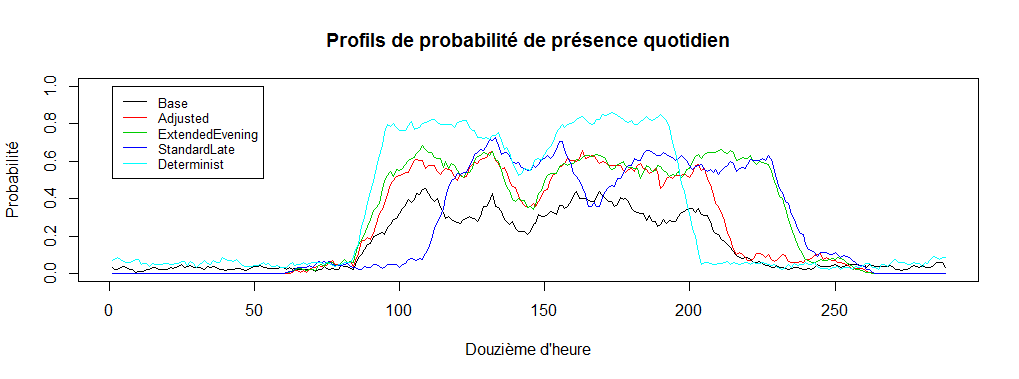
\includegraphics[scale=0.45]{Images/PageActivities/PresenceQ}
\caption{Profils de probabilité de présence quotidien moyens pour un agent simulé sur 1 année complète}
\label{fig:PresenceQ}
\end{figure}

\begin{figure}
\centering
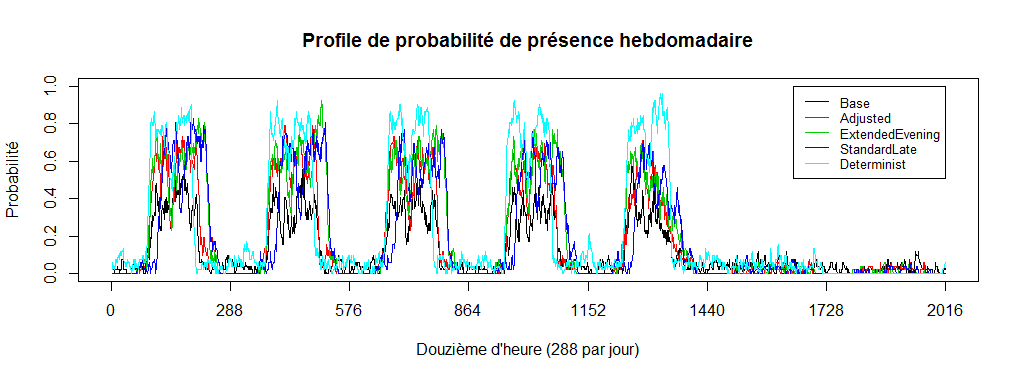
\includegraphics[scale=0.45]{Images/PageActivities/PresenceH}
\caption{Profils de probabilité de présence hebdomadaire moyens pour un agent simulé sur 1 année complète}
\label{fig:PresenceH}
\end{figure}

\begin{figure}
\centering
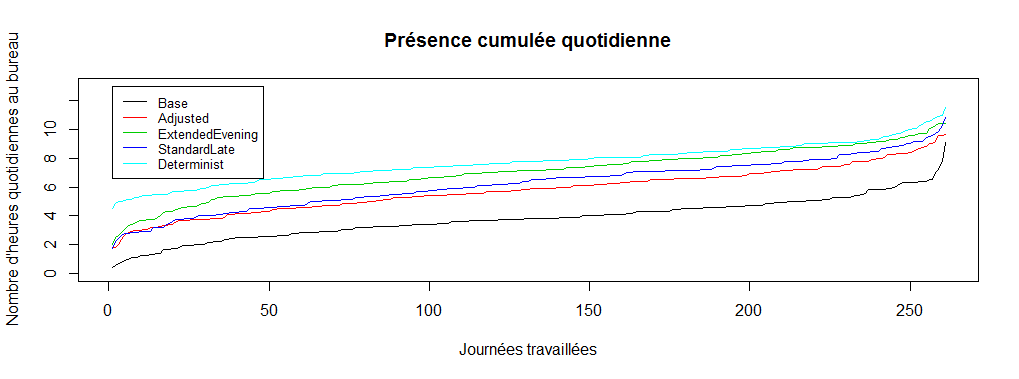
\includegraphics[scale=0.45]{Images/PageActivities/PresenceCumulee}
\caption{Distributions du nombre d'heures quotidiennes de présence pour un agent simulé sur 1 année complète}
\label{fig:PresenceCumulee}
\end{figure}

\begin{figure}
\centering
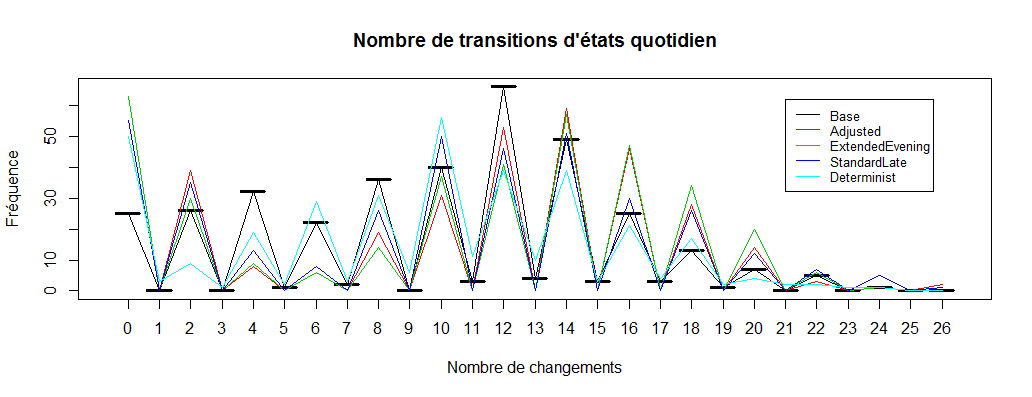
\includegraphics[scale=0.45]{Images/PageActivities/NbTransitions}
\caption{Distributions du nombre de transitions quotidien pour un agent simulé sur 1 année complète}
\label{fig:NbTransitions}
\end{figure}

\begin{figure}
\centering
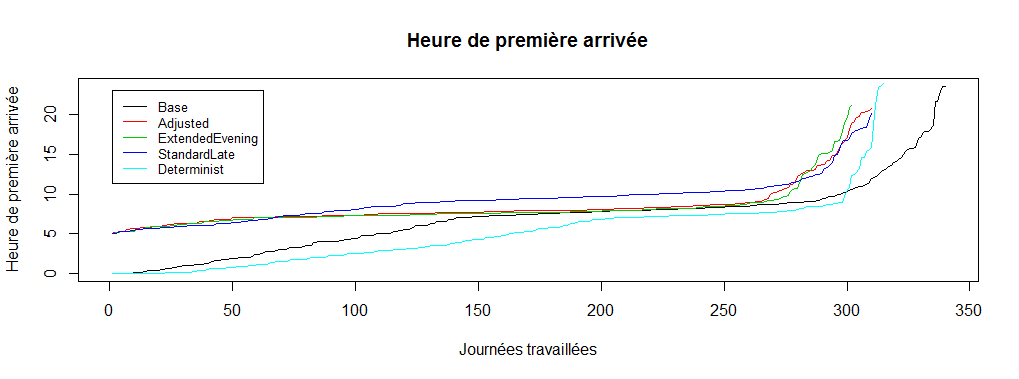
\includegraphics[scale=0.45]{Images/PageActivities/PremiereArrivee}
\caption{Distributions de l'heure de première arrivée dans le bureau pour un agent simulé sur 1 année complète}
\label{fig:PremiereArrivee}
\end{figure}

\begin{figure}
\centering
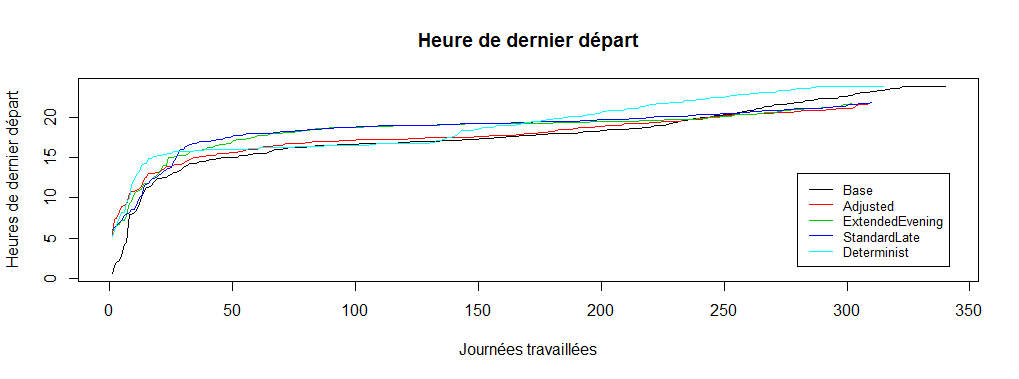
\includegraphics[scale=0.45]{Images/PageActivities/DernierDepart}
\caption{Distributions de l'heure de dernier départ dans le bureau pour un agent simulé sur 1 année complète}
\label{fig:DernierDepart}
\end{figure}

\newpage
\section{Activités dans les logements}
\label{ActivitésLogements}

Le fonctionnement général du modèle d'activités des logements est forcément très différent de celui des bureaux. Un point commun est qu'il est défini entièrement lors du pre-processus de la simulation. A la différence des bureaux, les activités dans les logements sont variées et ne sont donc pas limitées à la présence. Ces activités impliquent des comportements différents, des apports métaboliques différents dans les différentes zones du logement. La première partie de cette section présente l'état de l'art et plus particulièrement deux modèles qui nous ont interpellé et que nous avons opposé. La seconde partie porte sur la présentation détaillée du modèle de Jaboob \cite{Jaboob-16} répondant à nos exigences avec parcimonie. Le modèle idéal comporte un nombre de paramètres d'entrée limité, il rend compte de la diversité des activités en fonction du type d'habitants et produit des profils d'activités différents pour des individus semblables. Un modèle d'activités stochastique dans les logements convient alors parfaitement à la nature stochastiques des comportements humains.

\subsection{État de l'art}

L'état de l'art a permis de déterminer que l'ensemble des modèles d'activités proposés se base sur des enquêtes emploi du temps. Ces enquêtes se basent sur des échantillons de population larges (de l'ordre de 10000 participants) qui assurent une bonne représentativité des comportements de la vie quotidienne. Chaque répondant d'une enquête est associé à un descriptif socio-démographique et un carnet d'activités renseigné précisément sur une ou plusieurs journées. Le traitement de ces résultats permet de confronter les activités en cours avec les caractéristiques des individus. Ce traitement de données a mené à plusieurs modèles élaborés par Tanimoto et al. \cite{Tanimoto-08}, Widèn et al. \cite{Widen-12} ou encore Aerts et al. \cite{Aerts-14}, sans être exhaustif. Nous proposons dans la suite de détailler deux modèles qui ont particulièrement attirés notre attention, celui de Wilke et al. \cite{Wilke-13} et celui de Jaboob \cite{Jaboob-16}.

Vorger \cite{Vorger-14} reprend la stratégie de modélisation des activités dans les logements de Wilke et al. \cite{Wilke-13}. La base de données utilisée est issue de l'étude de 1998-1999\footnote{L'Enquête Emploi du Temps (EET) n'est plus disponible en ligne et a été remplacée par l'enquête plus récente de 2009-2010} de l'INSEE sur 7949 ménages et 15441 individus français qui ont noté leurs activités sur une journée toutes les 10 minutes. Le modèle proposé issu de cet EET permet dans une première étape de générer pour chaque occupant des périodes de présence et d'absence. Lorsqu'une période de présence débute, une des 20 activités débute également, suivant un modèle de Markov, et une durée lui est attribuée, suivant une loi de Weibull. Si l'activité prend fin avant la période d'absence alors une autre activité débute. En revanche, si une période d'absence commence avant la fin de l'activité alors cette dernière est abrogée. Les modèles de Markov et Weibull sont influencés par l'heure de la journée, par des caractéristiques du ménage et par des caractéristiques individuelles des occupants, rendant les profils d'activités très spécifique à chaque occupant. On peut néanmoins noter que ce modèle hybride présente quelques légers point d'amélioration à apporter. En effet, en raison de la non-continuité de l'enquête emploi du temps à minuit, les activités sont interrompus chaque jour à minuit conduisant à un début de période de sommeil quasi général à minuit et très rarement avant minuit. L'enquête datant de 1999, on peut également se demander si l'évolution des pratiques n'est pas suffisamment significative pour considérer une mise à jour. Aussi, le nombre de vingt activités renseignées nous semble excessif pour un exercice de modélisation de la performance énergétique.

Jaboob \cite{Jaboob-16} a plus récemment proposé un nouveau modèle d'activités basé sur une enquête emploi du temps anglaise datant de 2000-2001. La base de données est issue de questionnaires également renseignés toutes les 10 minutes sur une journée par 6500 ménages et 11700 individus. A partir de ces données, 10 modèles ont été développés et comparés. Il est conclu que le modèle de hybride Markov + Weibull fonctionne le mieux mais que le modèle de Bernoulli seul est recommandé pour sa simplicité et son faible nombre de paramètre d'entrées (240 contre 2880) tout en étant que très légèrement moins performant que le modèle hybride. Sur la base de ces conclusions, Chapman \cite{Chapman-16} utilise pour la prédiction des activités résidentiels ce modèle parcimonieux de Bernoulli, celui-ci ayant été recommandé. La qualité des modèles a été jugé en se basant sur 5 critères de validation et d'évaluation: 
\begin{itemize}
\item la sensibilité qui évalue la capacité du modèle à donner un résultat positif lorsqu'une hypothèse est vérifiée
\item la spécificité qui évalue la capacité du modèle à donner un résultat négatif lorsque l'hypothèse n'est pas vérifiée.
\item la précision qui regroupe la sensibilité et la spécificité
\item l'écart moyen à la moyenne, qui évalue l'amplitude de la différences de probabilité entre les simulations et les mesures.
\item l'indice de Brier, qui évalue la précision des probabilités du modèle
\end{itemize}

Or, nous notons qu'aucun de ces paramètres n'évalue le nombre de transitions d'état, qui nous semble pourtant fondamental pour reproduire des emplois du temps probables. Pour cette raison, il nous semble plus approprié d'utiliser un modèle d'activités hybride qui associe à chaque activité commencée une durée. Mahdavi et Tahmasebi \cite{Mahdavi-15} proposent un indicateur, sans unité, qu'ils appellent erreur du nombre de transitions et qui est défini par le nombre de transitions prédit moins le nombre de transitions mesurées. Ne possédant pas la base de donnée utilisée par Jaboob pour le développement du modèle, nous proposons dans la suite de simplement calculer le nombre de transitions d'état par jour issu des modèles et de les comparer.

\subsection{Processus de Bernoulli}

A partir de l'EET Anglaise, Jaboob \cite{Jaboob-16} propose un modèle permettant de générer 10 activités. En pré-processus, le modèle calcule pour chaque pas de temps l'activité réalisée pour les occupants. Le Tableau \ref{tab:Activités} les synthétise et associe à chaque activité le lieu où elles se produisent et l'état de l'occupant associé.

La diversité entre agents impacte leurs activités. Les variables explicatives des activités dans les logements sont relatives aux occupants (age, statut civique, genre, retraité/actif, chômeur/actif, niveau éducatif), au ménage (situation familiale, possession d'un ordinateur) et à l'environnement (heure de la journée, jour, saison). Le Tableau \ref{VariablesActivité} détaille ces variables et leurs différents niveaux.

\begin{table} [H]
\centering
\begin{tabular}{|p{5 cm}||p{5 cm}|p{5 cm}|}
\hline Activités & Localisation & État de l'occupant (Clo et Met [$W/m^{2}$]) \\
\hline
\hline 0- Dormir & Chambre & Clo = 2.55 \newline Met = 46 \\
\hline 1- Passif & Salon & Clo = 1 \newline Met = 58 \\
\hline 2- Audio-visuel & Salon & Clo = 1 \newline Met = 70 \\
\hline 3- Bureautique & Bureau ou chambre & Clo = 1 \newline Met = 116 \\
\hline 4- Cuisine & Cuisine & Clo = 1 \newline Met = 116 \\
\hline 5- Nettoyage & Cuisine & Clo = 1 \newline Met = 116 \\
\hline 6- Toilette corporelle & Salle de bain & Clo = 0 \newline Met = 116 \\
\hline 7- Vaisselle et machine à laver & Cuisine & Clo = 1 \newline Met = 93 \\
\hline 8- Bricolage & Salon & Clo = 1 \newline Met = 93 \\
\hline 9- Absent & Extérieur & .  \\
\hline
\end{tabular}
\normalsize
\caption{Nature des activités et états associés}
\label{tab:Activités}
\end{table}

\begin{table} [H]
\centering
\begin{tabular}{|p{4 cm}||p{11 cm}|}
\hline Variables & Niveaux - \textit{Codes} \\
\hline
\hline Age & Plus de 59 ans - \textit{age1} \newline Entre 36 et 59 and - \textit{age2} \newline Moins de 36 ans - \textit{age3} \\
\hline Statut civique & En couple (marié, concubinage, partenaire civique) - \textit{civstat1} \newline Célibataire - \textit{civstat2} \\
\hline Genre & Homme - \textit{sex1} \newline Femme - \textit{sex2} \\
\hline Retraité & Actif - \textit{retired0} \newline Retraité - \textit{retired1} \\
\hline Chômeur & Actif - \textit{unemp0} \newline Chômeur - \textit{unemp1} \\
\hline Éducation & Lycée ou moins - \textit{edtry1} \newline Premier cycle - \textit{edtry2} \newline Second cycle et plus - \textit{edtry3}  \\
\hline Situation familiale & Adulte(s) sans enfants - \textit{famstat0} \newline Adulte(s) avec bébé (moins de 5 ans) - \textit{famstat1} \newline Adulte(s) avec enfants (entre 5 et 18 ans) - \textit{famstat2} \newline Adulte de plus de 40 ans sans enfants - \textit{famstat3} \newline Enfant avec parents ou garde - \textit{famstat4} \newline Enfant sans parents ou garde - \textit{famstat5} \\
\hline Possession d'ordinateur & Non - \textit{computer0} \newline Oui - \textit{conputer1} \\
\hline Heure & \textit{1 - 24} \\
\hline Jour & Lundi : Dimanche - \textit{day1} : \textit{day7} \\
\hline Saison & Printemps - \textit{season1} \newline Eté - \textit{season2} \newline Automne - \textit{season3} \newline Hiver - \textit{season4} \\
\hline
\end{tabular}
\normalsize
\caption{Variables sélectionnées pour expliquer les activités des occupants}
\label{VariablesActivité}
\end{table}

L'équation ci-dessous, issue de la régression logistique multinomial de l'EET, permet de calculer la probabilité, $P_{j}(x,t)$ de commencer une nouvelle activité.

\begin{equation}
P_{j}(x,t)=\frac{exp(A_{j}(x))}{\sum\limits_{j=1}^{N}exp(A_{j}(x))}, j = 1, .., N et A_{j}(x)= \alpha_{j}+\sum\limits_{k=1}^{n}\beta_{jk}x_{jk}
\end{equation}

N correspond au nombre d'activités total, soit 10, n correspond au nombre de prédicteurs, soit 10 (nombre de variables dans le Tableau \ref{VariablesActivité} excepté l'heure), $\alpha$ et $\beta$ sont respectivement l'interception et la pente. Les probabilités de commencer une activité dépendent ainsi des caractéristiques des occupants mais également du temps, en émane donc pour chaque occupant une matrice à 4 dimensions [10][24][7][4] (activités, heures, jour de la semaine et saison, respectivement).

\subsection{Modèle hybride}

Le modèle hybride couple au modèle de Bernoulli un modèle de Weibull. Ainsi, lorsqu'une activité débute, une durée correspondante y est associée. Wilke propose dans son modèle d'activités des coefficients de durée désagrégés. Bien sûr, les fonctions de Weibull diffèrent temporellement, la durée de l'activité de sommeil est plus longue si elle commence en début de nuit qu'en début d'après-midi, mais elle diffèrent également selon les caractéristiques des occupants, la durée d'un repas pour un retraité est plus longue que pour un actif. Pour considérer ces caractéristiques liées aux occupants les données sont structurées en arbres binaires. Pour chaque activité et chaque heure de la journée un arbre binaire est proposé, les nœuds de celui-ci étant formé par les attributs des occupants.

Au contraire, Jaboob \cite{Jaboob-16} fourni dans sa thèse les coefficients de forme et d'échelle de manière agrégés pour chaque heure et activité de la simulation, mais pas en fonction des caractéristiques des occupants. L'auteur justifie ce choix par un modèle davantage parcimonieux et une plus-value discutable de la désagrégation, les distinctions étant très peu intuitives et les caractéristiques des individus  multi-colinéaires. Pour ces raisons, nous décidons d'utiliser les coefficients agrégés de Jaboob.

La durée de l'équation est alors définie par l'équation ci-dessous, U étant un nombre aléatoire tiré entre 0 et 1. 

\begin{equation}
t_{j}=\frac{(-log(U))^{\frac{1}{k}}}{\lambda}
\end{equation}

Les paramètres de forme $k$ et d'échelle $\lambda$, déterminés par la méthode du maximum de vraisemblance, maximisent la probabilité de reproduire, par une loi de Weibull, la distribution observée de l'enquête emploi du temps.

Il est à noter que les coefficients de la loi de Weibull ne sont pas connus pour l'activité informatique (\textit{IT}) lorsqu'elle a lieu de 2 à 4 heures du matin dans la base de donnés de Jaboob. Cela est la conséquence d'un événement peu ou pas présent à ces heures dans la base de données. Pour s'affranchir de cette méconnaissance problématique pour le modèle, nous proposons une simple interpolation linéaire basée sur les intervalles de temps précédent et suivant:
\begin{equation}
f(x)=\frac{x_{b}-x}{x_{b}-x_{a}}y_{a}+\frac{x-x_{a}}{x_{b}-x_{a}}y_{b}
\end{equation}
Sachant que $\lambda(2)=61.806$ et que $\lambda(5)=40.125$ on a alors $\lambda(3)=54.579$ et $\lambda(4)=47.352$. Et sachant que $k(2)=1.143$ et que $k(5)=0.813$ on a alors $k(3)=1.033$ et $k(4)=0.923$. L'ensemble des coefficients se trouve en Annexe de la thèse de Jaboob \cite{Jaboob-16}.

\subsection{Présentation des résultats}

Afin de tester et visualiser les sorties des modèles d'activités dans les logements, nous avons généré un ensemble de graphiques, Figure \ref{fig:Activités}, qui présente les profils d'activités journaliers de 2 occupants différents, le premier est un jeune homme de 20 ans, avec ordinateur, actif et célibataire alors que le second est un retraité marié de 60 ans, sans ordinateur, sous les deux types de modèles, Bernoulli et hybride. Les profils générés par les deux familles de modèle sont globalement en accord avec le sens commun, nous pouvons néanmoins émettre un certain nombre de critiques. Pour la comparaison d'archétype, on retrouve sans surprise une proportion de temps à l'extérieur très supérieur chez l'occupant actif que chez le retraité, une durée devant la télévision supérieure pour le retraité ou encore une période de sieste plus significative chez les retraités. Étonnamment, plusieurs activités sont réparties uniformément sur la période d'éveil, comme l'activité cuisine dont on attendait des pics aux heures de repas. Également étonnamment, on note une importante proportion de l'activité informatique à 9 et 14 heure chez l'occupant retraité. Pour la comparaison des deux modèles on a tendance à penser que le modèle hybride reproduit mieux le sommeil que le modèle de Bernoulli qui génère assez peu d'heures de sommeil et un nombre d'autres activités semble t-il élevé. L'activité douche-toilette se retrouve dans le modèle hybride quant à elle réduite mais les deux pics du matin et du soir restent visibles.

La Figure \ref{fig:ExempleScenario} permet d'évaluer le nombre de transitions entre deux activités. Sans surprise, nous ne notons pas de différences significatives entre le nombre de transitions entre deux catégories d'occupants, au contraire du type de modèle. Sur 150 jours de simulations, le modèle de Bernoulli a généré en moyenne 185 activités quotidienne contre 56 pour le modèle hybride, pour un pas de temps de 5 minutes. Cet indicateur est difficile à interpréter rigoureusement car nous n'avons pas identifié de valeur étalonnée dans la littérature. En effet, l'enquête emploi du temps est à pas de temps fixe, plusieurs activités peuvent alors avoir lieu sur un même pas de temps sans être prise en compte dans l'enquête. Le nombre d'activités recensés dans l'enquête est également de grande influence sur le nombre de changement d'états. Enfin, le pas de temps de simulation, impacte considérablement ce nombre de transitions. Une simulation au pas de temps de 10 minutes a mené à 14 transitions, contre les 56 au pas de 5 minutes. Cet indicateur de nombre de transitions n'est en revanche pas sans intérêt, d'une part car il peut être utilisé pour comparer des modèles, ici le modèle de Bernoulli seul au modèle hybride Bernoulli (pour déterminer le début des activités) + Weibull (pour déterminer les durées des activités) et d'autres part pour mieux appréhender la dynamique des occupants dans ce modèle de prédiction des activités.

Comme nous l'avons indiqué en introduction, nous ne proposons pas pour le modèle d'activités dans les logements résidentiels d'adaptation contextuelle supplémentaire, car le modèle initial comporte de base 11 variables. Nous estimons donc que le développement de ce modèle a suffisamment bien intégré la diversité d'activité des occupants sans devoir à l'accentuer. 

\begin{figure}[H]
\centering
\begin{tabular}{cc}
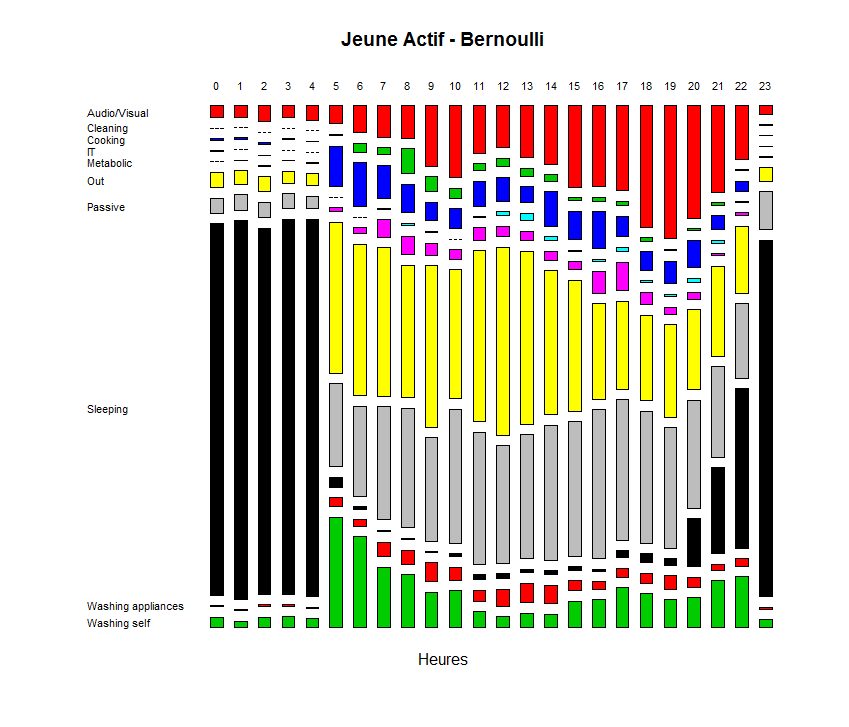
\includegraphics[scale=0.38]{Images/Activites/JeuneActifBernoulli} &
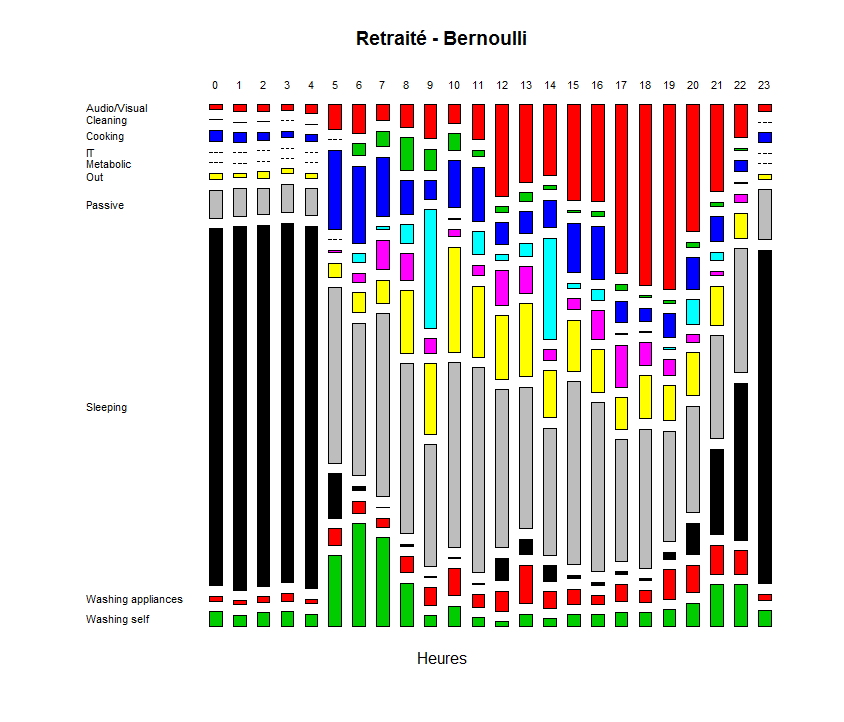
\includegraphics[scale=0.38]{Images/Activites/RetraiteBernoulli} \\
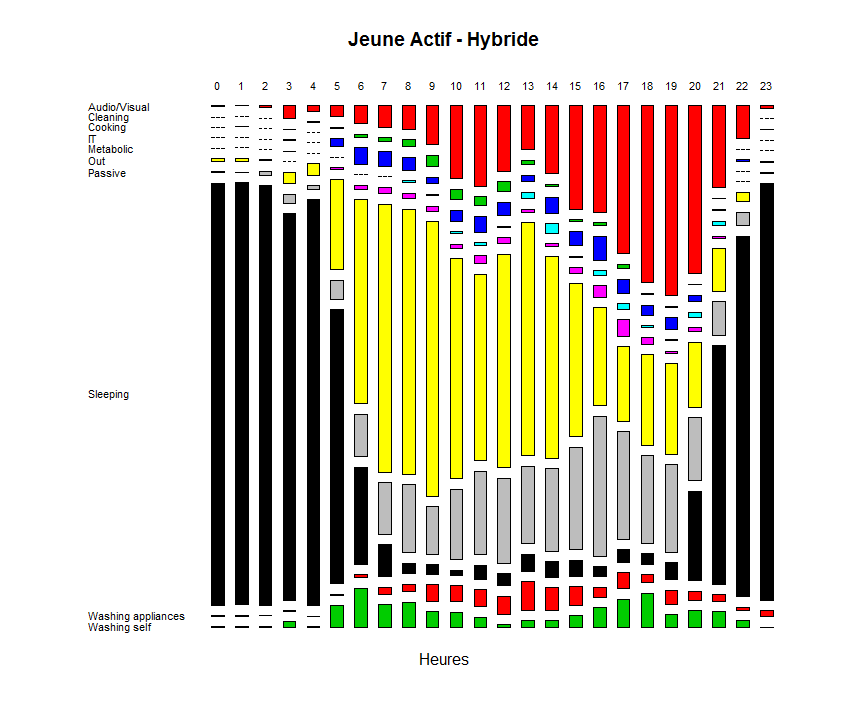
\includegraphics[scale=0.38]{Images/Activites/JeuneActifHybride} &
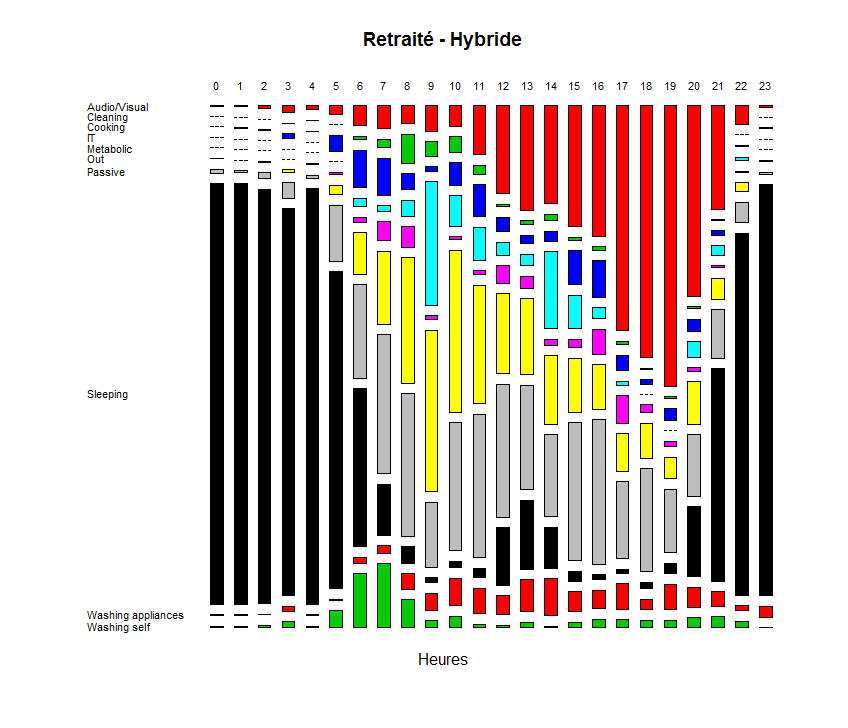
\includegraphics[scale=0.38]{Images/Activites/RetraiteHybride} \\
\end{tabular}
\caption{Chronogramme moyen des activités sur une journée calculé sur 150 jours, pour un jeune actif (à gauche) et pour un retraité (à droite), selon le modèle de Bernoulli (en haut) et le modèle hybride Bernoulli + Weibull(en bas), toutes choses égales par ailleurs}
\label{fig:Activités}
\end{figure}

\begin{figure}[H]
\centering
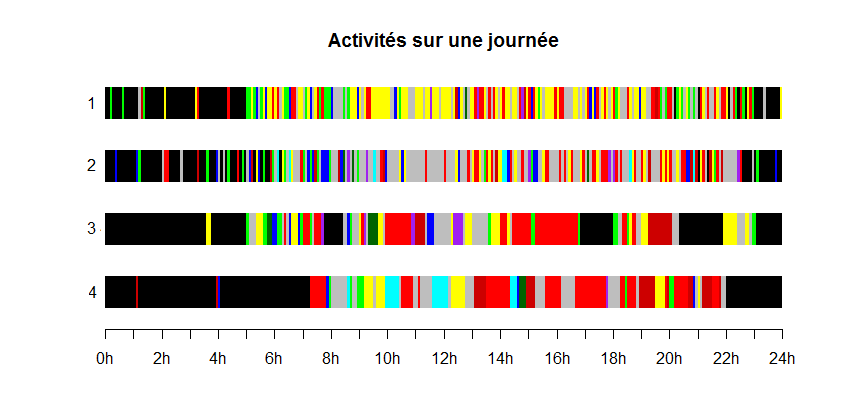
\includegraphics[scale=0.7]{Images/Activites/ActivitesSurUneJournee}
\caption{Exemple de scénarios d'activités pour une journée d'hiver pour; 1- l'actif avec le modèle de Bernoulli, 2- le retraité avec le modèle de Bernoulli, 3- l'actif avec le modèle hybride, 4- le retraité avec le modèle hybride. Le code couleur est le même que pour la Figure \ref{fig:Activités}}
\label{fig:ExempleScenario}
\end{figure}
